\chapter{Der Simulator}

\section{Die grafische Anwenderschnittstelle}

\begin{figure}[htbp]
	\centering
	\fbox{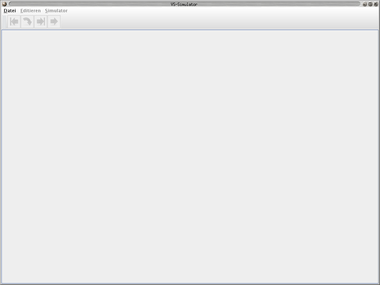
\includegraphics{images/ss-neues-fenster-klein}}
	\caption{Der Simulator nach dem ersten Starten}
	\label{fig:NeuesFenster}
\end{figure}

Der Simulator pr\"{a}sentiert sich nach dem ersten Starten wie auf Abbildung \ref{fig:NeuesFenster}. F\"{u}r die Erstellung einer neuen Simulation wird im Men\"{u} ``Datei'' (Abbildung \ref{fig:DateiMenue}) der Punkt ``Neue Simulation'' ausgew\"{a}hlt, wo anschlie�end das Einstellungsfenster f\"{u}r die neue Simulation erscheint.  Auf die einzelnen Optionen wird sp\"{a}ter genauer eingegangen und es werden nun nur die Standardeinstellungen \"{u}bernommen. Die GUI mit einer frischen Simulation sieht aus wie auf Abbildung \ref{fig:NeuErstellteSimulation}.

\begin{figure}[htbp]
	\centering
	\fbox{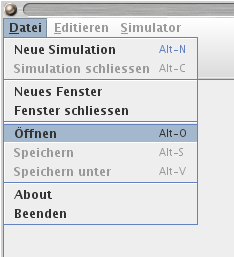
\includegraphics[width=14cm]{images/ss-datei-menu}}
	\caption{Datei-Men\"{u}}
	\label{fig:DateiMenue}
\end{figure}

\subsubsection{Die Men\"{u}zeile}

Im Datei-Men\"{u} (Abbildung \ref{fig:DateiMenue}) lassen sich neue Simulationen erstellen oder die aktuell ge\"{o}ffnete Simulation schlie�en. Neue Simulationen \"{o}ffnen sich standardm\"{a}�ig in einem neuen Tab. Es k\"{o}nnen allerdings auch neue Simulationsfenster, die wiederum eigene Tabs besitzen, ge\"{o}ffnet oder geschlossen werden. In jedem Tab befindet sich eine von den Anderen vollst\"{a}ndig unabh\"{a}ngige Simulation. Es k\"{o}nnen somit beliebig viele Simulationen parallel ausgef\"{u}hrt werden. Die Men\"{u}eintr\"{a}ge ``\"{O}ffnen'', ``Speichern'' und ``Speichern unter'' dienen f\"{u}r das Laden und Speichern von Simulationen. 

\begin{figure}[htbp]
	\centering
	\fbox{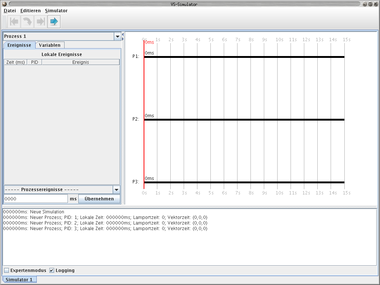
\includegraphics{images/ss-neue-simulation-klein}}
	\caption{Eine neue Simulation}
	\label{fig:NeuErstellteSimulation}
\end{figure}

\"{U}ber das Editieren-Men\"{u} gelangt der Anwender zu den Simulationseinstellungen, worauf sp\"{a}ter genauer eingegangen wird. Es werden in diesem Men\"{u} auch alle beteiligten Prozesse zum Editieren aufgelistet. W\"{a}hlt der Anwender dort einen Prozess aus, dann \"{o}ffnet sich der dazugeh\"{o}rige Prozesseditor. Auf diesen wird ebenso sp\"{a}ter genauer eingegangen. Das Simulator-Men\"{u} bietet die selben Optionen wie die Toolbar, welche im n\"{a}chsten Teilkapitel beschrieben wird, an.

Einige Men\"{u}unterpunkte sind erst erreichbar, wenn im aktuellen Fenster eine Simulation erstellt oder geladen wurde.

\subsubsection{Die Toolbar}

Oben links im Simulator befindet sich die Toolbar (Abbildung \ref{fig:Toolbar}). Die Toolbar enth\"{a}lt die Funktionen die vom Anwender am h\"{a}ufigsten ben\"{o}tigt werden.

\begin{figure}[htbp]
	\centering
	\fbox{
\includegraphics[width=5cm]{images/ss-neue-simulation-toolbar}}
	\caption{Die Men\"{u}zeile inklusive Toolbar}
	\label{fig:Toolbar}
\end{figure}

Die Toolbar bietet vier verschiedene Funktionalit\"{a}ten an:

\begin{itemize}
	%\setlength{\itemsep}{-1mm}
	\item Starten der Simulation; kann nur bet\"{a}tigt werden, wenn die Simulation derzeit nicht l\"{a}uft.
	\item Pausieren der Simulation; kann nur bet\"{a}tigt werden, wenn die Simulation derzeit l\"{a}uft.
	\item Wiederholen der Simulation; kann nicht bet\"{a}tigt werden, wenn die Simulation noch nicht gestartet wurde. 
	\item Zur\"{u}cksetzen der Simulation; kann nur bet\"{a}tigt werden, wenn die Simulation pausiert wurde oder wenn die Simulation abgelaufen ist.
\end{itemize}

Die Toolbar l\"{a}sst sich nach Wunsch repositionieren (z.B. links, rechts oder unten des Simulatorfensters). Hierf\"{u}r muss sie per ``Drag-n-Drop'' zur Zielposition gezogen werden.

\subsubsection{Die Visualisierung}

\begin{figure}[htbp]
	\centering
	\fbox{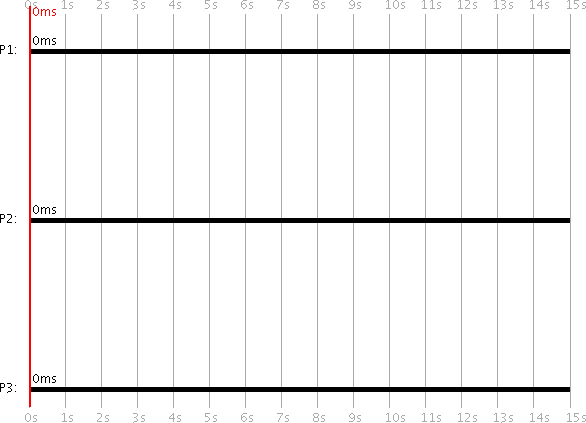
\includegraphics[width=14cm]{images/ss-visualisierung}}
	\caption{Visualisierung einer noch nicht gestarteten Simulation}
	\label{fig:Visualisierung}
\end{figure}

Mittig rechts befindet sich die grafische Simulationsvisualisierung. Die X-Achse gibt die Zeit in Millisekunden an und auf der Y-Achse sind alle beteiligten Prozesse aufgef\"{u}hrt. Unsere Demo-Simulation endet nach genau 15 Sekunden. Auf Abbildung \ref{fig:Visualisierung} sind 3 Prozesse (mit den PIDs 1, 2 und 3) dargestellt, die jeweils einen eigenen horizontalen schwarzen Balken besitzen. Auf diesen Prozessbalken kann der Anwender die jeweilige lokale Prozesszeit ablesen. Die vertikale rote Linie stellt die globale Simulationszeit dar. 

Die Prozessbalken dienen auch f\"{u}r Start- und Zielpunkte von Nachrichten. Wenn beispielsweise Prozess 1 eine Nachricht an Prozess 2 verschickt, so wird eine Linie vom einen Prozessbalken zum Anderen gezeichnet. Nachrichten, die ein Prozess an sich selbst schickt, werden nicht visualisiert. Sie werden aber im Loggfenster (mehr dazu sp\"{a}ter) protokolliert.

Eine andere M\"{o}glichkeit einen Prozesseditor aufzurufen ist ein Linksklick auf den zum Prozess geh\"{o}rigen Prozessbalken. Dies muss also nicht zwingend \"{u}ber das Simulator-Men\"{u} geschehen. Ein Rechtsklick hingegen \"{o}ffnet ein Popup-Fenster mit weiteren Auswahlm\"{o}glichkeiten (Abbildung \ref{fig:RechtsklickProzessbalken}). Ein Prozess kann \"{u}ber das Popup-Men\"{u} nur w\"{a}hrend einer laufenden Simulation zu einem Absturz oder einer Wiederbelebung bewegt werden.

\begin{figure}[htbp]
	\centering
	\fbox{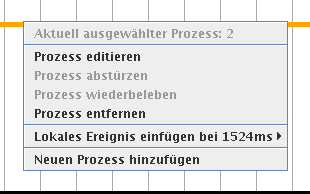
\includegraphics[width=8.8cm]{images/ss-rechtsklick-prozessbalken}}
	\caption{Rechtsklick auf einen Prozessbalken}
	\label{fig:RechtsklickProzessbalken}
\end{figure}

Generell kann die Anzahl der Prozesse nach belieben variieren. Die Dauer der Simulation betr\"{a}gt mindestens \texttt{5} und h\"{o}chstens \texttt{120} Sekunden. Die Simulation endet erst, wenn sie die globale Zeit die angegebene Simulationsendzeit (hier \texttt{15} Sekunden) erreicht hat, und nicht, wenn eine lokale Prozesszeit diese Endzeit erreicht. 

\subsubsection{Farbliche Differenzierung}

Farben helfen dabei die Vorg\"{a}nge einer Simulation besser zu deuten. Standardm\"{a}�ig werden die Prozesse (Prozessbalken) und Nachrichten mit den Farben wie in Tabelle \ref{tb:Farben} aufgelistet dargestellt. Dies sind lediglich die Standardfarben, welche \"{u}ber die Einstellungen ge\"{a}ndert werden k\"{o}nnen.

\begin{table}
	\fbox{
	\begin{tabular}{c|l}
		\textbf{Prozessfarbe} & \textbf{Bedeutung} \\
		\hline 
		 	Schwarz & Die Simulation l\"{a}uft derzeit nicht\\
				& pausiert)\\
		 	Orange & Die Maus befindet sich \"{u}ber den Prozessbalken\\
		 	Rot & Der Prozess ist abgest\"{u}rzt\\
			& \\
		\textbf{Nachrichtenfarbe} & \textbf{Bedeutung} \\
		\hline 
		 	Gr\"{u}n & Die Nachricht ist noch unterwegs und hat das Ziel noch nicht erreicht\\
		 	Blau & Die Nachricht hat das Ziel erfolgreich erreicht\\
		 	Rot & Die Nachricht ging verloren\\
	\end{tabular}\\
	}
	\caption{Farbliche Differenzierung von Prozessen und Nachrichten}
	\label{tb:Farben}
\end{table}

\subsubsection{Die Sidebar}

Mit Hilfe der Sidebar lassen sich Prozessereignisse programmieren. Oben auf Abbildung \ref{fig:Sidebar} ist der zu verwaltende Prozess selektiert (hier mit der PID 1). In dieser Prozessauswahl gibt es auch die M\"{o}glichkeit ``Alle Prozesse'' auszuw\"{a}hlen, womit die Ereignisse aller Prozesse gleichzeitig verwaltet werden k\"{o}nnen. Unter ``Lokale Ereignisse'' versteht man diejenigen Ereignisse, die auftreten, wenn eine bestimmte lokale Zeit des dazugeh\"{o}rigen Prozesses eingetreten ist. Die darunterliegende Ereignistabelle listet alle programmierten Ereignisse (hier noch keine vorhanden) mitsamt Eintrittszeiten sowie den PIDs auf.

\begin{figure}[htbp]
	\centering
	\fbox{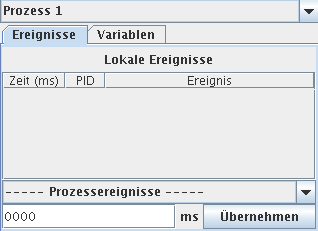
\includegraphics[width=9cm]{images/ss-sidebar}}
	\caption{Die Sidebar mit leerem Ereigniseditor}
	\label{fig:Sidebar}
\end{figure}

F\"{u}r die Erstellung eines neuen Ereignisses kann der Anwender entweder mit einem Rechtsklick auf einen Prozessbalken (Abbildung \ref{fig:RechtsklickProzessbalken}) klicken und dort ``Lokales Ereignis einf\"{u}gen'' w\"{a}hlen, oder unterhalb der Ereignistabelle ein Ereignis ausw\"{a}hlen (Abbildung \ref{fig:Ereignisauswahl}), im darunter liegendem Textfeld die Ereigniseintrittszeit eintragen und auf ``\"{U}bernehmen'' gehen. Beispielsweise wurden auf Abbildung \ref{fig:SidebarMitEreignissen} drei Ereignisse hinzugef\"{u}gt: Absturz nach \texttt{123ms}, Wiederbelebung nach \texttt{321ms} und erneuter Absturz nach \texttt{3000ms} des Prozesses mit der ID 1. 

\begin{figure}[htbp]
	\centering
	\fbox{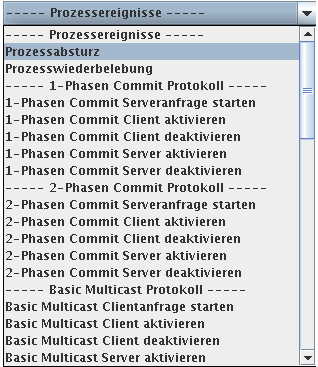
\includegraphics[width=9cm]{images/ss-ereignisauswahl}}
	\caption{Die Ereignisauswahl via Sidebar}
	\label{fig:Ereignisauswahl}
\end{figure}

Mit einem Rechtsklick auf den Ereigniseditor lassen sich alle selektierten Ereignisse entweder kopieren oder l\"{o}schen. Mit Hilfe der Strg-Taste k\"{o}nnen auch mehrere Ereignisse gleichzeitig markiert werden. Die Eintr\"{a}ge der Spalten f\"{u}r die Zeit und der PID lassen sich nachtr\"{a}glich editieren. Somit besteht eine komfortable M\"{o}glichkeit bereits programmierte Ereignisse auf eine andere Zeit zu verschieben oder einen anderen Prozess zuzuweisen. Allerdings sollte der Anwender darauf achten, dass er nach dem \"{A}ndern der Ereigniseintrittszeit die Enter-Taste bet\"{a}tigt, da sonst die \"{A}nderung unwirksam ist.

In der Sidebar gibt es neben dem Ereignis-Tab einen weiteren Tab ``Variablen''. Hinter diesem Tab verbirgt sich der Prozesseditor des aktuell ausgew\"{a}hlten Prozesses. Dort k\"{o}nnen alle Variablen des Prozesses editiert werden. Der Prozesseditor wird sp\"{a}ter genauer behandelt. 

\begin{figure}[htbp]
	\centering
	\fbox{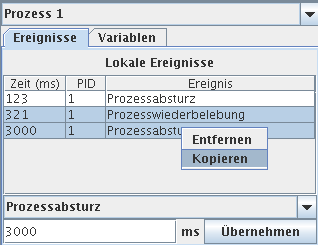
\includegraphics[width=9cm]{images/ss-sidebar-mit-ereignissen}}
	\caption{Der Ereigniseditor mit 3 programmierten Ereignissen}
	\label{fig:SidebarMitEreignissen}
\end{figure}

\subsubsection{Das Loggfenster}

Das Loggfenster (Abbildung \ref{fig:NeuErstellteSimulation}, unten) protokolliert  in chronologischer Reihenfolge alle eingetroffenen Ereignisse. Auf Abbildung \ref{fig:Loggfenster} sieht der Anwender das Loggfenster nach Erstellung unserer Simulation, an welcher 3 Prozesse beteiligt sind. Am Anfang eines Loggeintrages wird stets die globale Zeit in Millisekunden protokolliert. Bei jedem Prozess werden ebenso seine lokale Zeiten sowie die Lamport- und die Vektor-Zeitstempel aufgef\"{u}hrt. Letztere werden sp\"{a}ter genauer behandelt.  Hinter den Zeitangaben werden weitere Angaben, wie beispielsweise welche Nachricht mit welchem Inhalt verschickt wurde und welchem Protokoll sie angeh\"{o}rt, gemacht. Dies wird sp\"{a}ter noch anhand von Beispielen demonstriert.

\begin{figure}[htbp]
	\centering
	\fbox{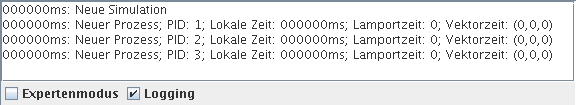
\includegraphics[width=16.5cm]{images/ss-loggfenster}}
	\caption{Das Loggfenster}
	\label{fig:Loggfenster}
\end{figure}

Mit dem Deaktivieren der Checkbox ``Logging'' l\"{a}�t sich das Loggen von Nachrichten tempor\"{a}r einstellen. Mit deaktiviertem Loggen werden keine neuen Nachrichten mehr ins Loggfenster geschrieben. Nach Reaktivieren der Checkbox werden alle ausgelassenen Nachrichten nachtr\"{a}glich in das Fenster geschrieben. Ein deaktiviertes Loggen kann zu verbessertem Leistungsverhalten des Simulators f\"{u}hren (z.B. kein Rucklen; ist vom verwendeten Computer, auf dem der Simulator l\"{a}uft, abh\"{a}ngig). Dieser Umstand ist der sehr langsamen Java-Implementierung der JTextArea-Klasse zu verdanken, die schnelle Updates nur sehr tr\"{a}ge durchf\"{u}hrt.

\"{U}ber die Checkbox ``Expertenmodus'' wird der Expertenmodus aktiviert beziehungsweise deaktiviert. 

\section{Der Expertenmodus}

\begin{figure}[htbp]
	\centering
	\fbox{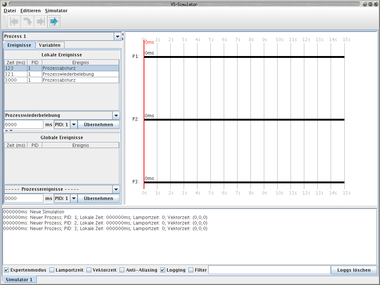
\includegraphics{images/ss-simulation-expertenmodus-klein}}
	\caption{Der Simulator im Expertenmodus}
	\label{fig:SimulationExpertenmodus}
\end{figure}

Der Simulator kann in zwei verschiedenen Modi betrieben werden. Es gibt einen einfachen- und einen Expertenmodus. Der Simulator startet standardm\"{a}�ig im einfachen Modus, sodass sich der Anwender nicht mit der vollen Funktionalit\"{a}t des Simulators auf einmal auseinandersetzen mu�. Der einfache Modus ist \"{u}bersichtlicher, bietet jedoch weniger Funktionen an. Der Expertenmodus eignet sich f\"{u}r mehr erfahrene Anwender und bietet dementsprechend auch mehr Flexibilit\"{a}t. Der Expertenmodus kann \"{u}ber die gleichnamige Checkbox unterhalb des Loggfensters oder \"{u}ber die Simulationseinstellungen aktiviert oder deaktiviert werden.  Auf Abbildung \ref{fig:SimulationExpertenmodus} ist der Simulator im Expertenmodus zu sehen. Wenn der Anwender den Simulator im Expertenmodus mit Abbildung \ref{fig:NeuErstellteSimulation} vergleicht, dann fallen einige Unterschiede auf, die nun behandelt werden.

\begin{figure}[htbp]
	\centering
	\fbox{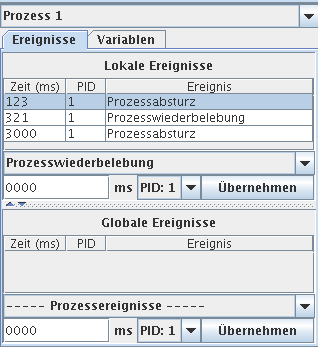
\includegraphics[width=9cm]{images/ss-sidebar-expertenmodus}}
	\caption{Die Sidebar im Expertenmodus}
	\label{fig:SidebarExpertenmodus}
\end{figure}

\subsubsection{Neue Funktionen in der Sidebar}

Der erste Unterschied ist in der Sidebar erkennbar (Abbildung \ref{fig:SidebarExpertenmodus}). Dort sind nun, zus\"{a}tzlich den lokalen Ereignissen, auch globale Ereignisse editierbar.  Wie bereits erw\"{a}hnt, sind unter lokale Ereignisse diejenigen Ereignisse zu verstehen, die auftreten, wenn eine bestimmte lokale Zeit des dazugeh\"{o}rigen Prozesses eingetreten ist. Globale Ereignisse hingegen sind diejenigen Ereignisse, die auftreten, wenn eine bestimmte globale Zeit eingetreten ist. Ein globales Ereignis nimmt die globale Zeit- und ein lokales Ereignis die lokale Prozesszeit als Eintrittskriterium. Globale Ereignisse machen somit nur einen Unterschied, wenn sich die lokalen Prozesszeiten von der globalen Zeit unterscheiden.

Eine weitere neue Funktionalit\"{a}t ist die M\"{o}glichkeit einem neuzuerstellenen Ereignis die PID direkt zuzuweisen. Im einfachen Modus wurde, wenn der Anwender ein neues Ereignis erstellte, standardm\"{a}�ig immer die PID des aktuell (in der obersten Combo-Box) ausgew\"{a}hlten Prozesses verwendet. In dieser Combo-Box sollte der Anwender gegebenenfalls ``Alle Prozesse'' selektieren, damit im Ereigniseditor stets die Ereignisse aller Prozesse aufgelistet werden.

\subsubsection{Lamportzeit, Vektorzeit und Anti-Aliasing Schalter}

Weitere Unterschiede machen sich unterhalb des Loggfensters bemerkbar. Dort gibt es unter Anderem zwei neue Checkboxen ``Lamportzeit'' und ``Vektorzeit''.  Aktiviert der Anwender eine dieser beiden Checkboxen, so wird die Lamport- beziehungsweise Vektorzeit in die Visualisierung dargestellt. \"{U}bersichtshalber kann der Anwender nur jeweils eine dieser beiden Checkboxen aktivieren. Wenn die Lamportzeit-Checkbox bereits aktiviert ist und der Anwender versucht die Vektorzeit-Checkbox zus\"{a}tzlich zu aktivieren, so wird die Lamportzeit-Checkbox automatisch deaktiviert und virce versa. 

Die Anti-Aliasing-Checkbox erm\"{o}glicht dem Anwender Anti-Aliasing zu aktivieren und deaktivieren. Mit aktiviertem Anti-Aliasing werden alle Grafiken der Visualisierung gerundet dargestellt. Aus Performancegr\"{u}nden ist Anti-Aliasing standardm\"{a}�ig nicht aktiv.

\subsubsection{Der Loggfilter}

Je komplexer eine Simulation wird, desto un\"{u}bersichtlicher werden die Eintr\"{a}ge im Loggfenster. Hier f\"{a}llt es zunehmend schwerer die \"{U}bersicht aller Ereignisse zu behalten. Um dem entgegenzuwirken gibt es im Expertenmodus einen Loggfilter, welcher es erm\"{o}glicht nur die wesentlichen Daten aus den Loggs zu filtern. Der Loggfilter wird anhand der dazugeh\"{o}rigen Checkbox ``Filter'' aktiviert beziehungsweise deaktiviert. In der dahinterliegenden Eingabezeile kann ein regul\"{a}rer Ausdruck in Java-Syntax angegeben werden. Beispielsweise werden mit ``\texttt{PID: (1|2)}'' nur Loggzeilen angezeigt, die entweder ``\texttt{PID: 1}'' oder ``\texttt{PID: 2}'' beinhalten. Alle anderen Zeilen, die zum Beispiel nur ``\texttt{PID: 3}'' beinhalten, werden dabei nicht angezeigt. Mit aktivem Loggfilter werden nur die Loggzeilen angezeigt, auf die der regul\"{a}re Ausdruck passt. Der Loggfilter kann auch nachtr\"{a}glich aktiviert werden, da bereits protokollierte Ereignisse nach jeder Filter\"{a}nderung erneut gefiltert werden. Der Loggfilter kann auch w\"{a}hrend einer laufenden Simulation verwendet werden. Wenn der Loggfilter deaktiviert wird, dann werden wieder alle Nachrichten (auch nachtr\"{a}glich) im Loggfenster angezeigt. 

\section{Ereignisse}

Es wird zwischen zwei verschiedenen Haupttypen von Ereignissen unterschieden: Programmierbare Ereignisse und nicht-programmierbare Ereignisse. Programmierbare Ereignisse lassen sich im Ereigniseditor editieren und deren Eintrittszeiten h\"{a}ngen von den lokalen Prozessuhren oder der globalen Uhr ab. Nicht-programmierbare Ereignisse lassen sich hingegen nicht im Ereigniseditor angeben und treten nicht wegen einer bestimmten Uhrzeit ein, sondern aufgrund anderer Gegebenheiten wie in etwa das Eintreffen einer Nachricht oder das Ausf\"{u}hren einer Aktion aufgrund eines Weckers, worauf weiter unten nochmal genauer eingegangen wird.

\subsubsection{Prozessabsturz- und Wiederbelebung (programmierbar)}

Die beiden grundliegensten Ereignisse sind ``Prozessabsturz'' sowie ``Prozesswiederbelebung''. Wenn ein Prozess abgest\"{u}rzt ist, so wird sein Prozessbalken in rot dargestellt. Ein abgest\"{u}rzter Prozess kann keine weiteren Ereignisse mehr verarbeiten und, wenn er eine Nachricht empfangen sollte, geht diese verloren. Die einzige Ausnahme bildet ein Wiederbelebungsereignis. Ein abgest\"{u}rzter Prozess kann nichts, au�er wiederbelebt werden. W\"{a}hrend eines Prozessabsturzes l\"{a}uft die lokale Prozessuhr, abgesehen der Lamport- und Vektor-Uhren, wie gewohnt weiter. Das hei�t es besteht die M\"{o}glichkeit, dass ein Prozess einige seiner Ereignisse gar nicht ausf\"{u}hrt, da er zu den Ereigniseintrittszeiten abgest\"{u}rzt ist. Wenn im echten Leben ein Computer abst\"{u}rzt oder abgeschaltet wird, dann l\"{a}uft dort die Hardware-Uhr, unabh\"{a}ngig vom Betriebssystem, auch weiter.

\subsubsection{Aktivierung und Deaktivierung von Protokollen sowie Starten von Anfragen (programmierbar)}
Wir wissen bereits, dass ein Prozess mehrere Protokolle Client- und auch Serverseitig unterst\"{u}tzen kann. Welches Protokoll von einem Prozess unterst\"{u}tzt wird, kann der Anwender anhand von Protokollaktivierungs- und Protokolldeaktivierungsereignissen konfigurieren. Somit besteht die M\"{o}glichkeit, dass ein gegebener Prozess ein bestimmtes Protokoll erst zu einem bestimmten Zeitpunkt unterst\"{u}tzt und gegebenenfalls ein anderes Protokoll abl\"{o}st. Jedes Protokoll kann entweder Server- oder Clientseitig aktiviert beziehungsweise deaktiviert werden. Welche Protokolle es gibt wird sp\"{a}ter behandelt. Der Anwender hat die Auswahl zwischen f\"{u}nf verschiedenen Protokollereignistypen: 

\begin{itemize}
	\item Aktivierung des Clients eines gegebenen Protokolls
	\item Aktivierung des Servers eines gegebenen Protokolls
	\item Deaktivierung des Clients eines gegebenen Protokolls
	\item Deaktivierung des Servers eines gegebenen Protokolls
	\item Starten einer Client/Server-Anfrage eines gegebenen Protokolls
\end{itemize}

Ob sich das Ereignis f\"{u}r das Starten einer Anfrage auf einen Client oder einen Server bezieht h\"{a}ngt vom verwendeten Protokoll ab. Es gibt Protokolle, wo der Client die initiale Anfrage starten muss, und es gibt Protokolle, wo der Server diese Aufgabe \"{u}bernimmt. Beispielsweise startet bei dem ``Ping-Pong Protokoll'' der Client- und bei dem ``Commit-Protokollen'' der Server immer die erste Anfrage. Es gibt kein Protokoll, wo Client und Server jeweils eine initiale Anfragen starten k\"{o}nnen. 

Bei allen dieser f\"{u}nf Ereignissen kann der betroffene Prozess noch beliebig andere Dinge, abh\"{a}ngig vom Protokoll, tun. Beispielsweise kann er den Inhalt der Nachricht generieren oder lokale Variablen initialisieren oder eine der lokalen Uhzeiten \"{a}ndern oder Wecker f\"{u}r ``Callback Ereignisse'' setzen (mehr dazu sp\"{a}ter) und vieles mehr.

\subsubsection{Nachrichtenempfang sowie Antwortnachrichten (nicht-programmierbar)}

Nachdem ein Prozess eine Nachricht empf\"{a}ngt wird zuerst \"{u}berpr\"{u}ft ob er das dazugeh\"{o}rige Protokoll unterst\"{u}tzt. Wenn der Prozess das Protokoll unterst\"{u}tzt, wird geschaut ob es sich um eine Client- oder eine Servernachricht handelt. Wenn es sich um eine Clientnachricht handelt, so mu� der Empf\"{a}ngerprozess ein das Protokoll serverseitig unterst\"{u}tzen und virce versa. Wenn alles passt, dann f\"{u}hrt der Empf\"{a}ngerprozess die vom Protokoll definierten Aktionen aus. In der Regel berechnet der Prozess irgendeinen Wert und schickt ihn \"{u}ber eine Antwortnachricht zur\"{u}ck. Es k\"{o}nnen aber auch beliebig andere Aktionen ausgef\"{u}hrt werden. Welche dies sind h\"{a}ngt vom Protokoll ab.

\subsubsection{Callback-Ereignisse (nicht-programmierbar)}

Ein Callback-Ereignis kann von einem Protokoll ausgel\"{o}st werden. Das Protokoll setzt einen Wecker, der angibt zur welcher lokalen Uhrzeit eine weitere Aktion ausgef\"{u}hrt werden soll. Zum Beispiel lassen sich hiermit Timeouts realisieren: Wenn ein Protokoll eine Antwort erwartet, diese aber nicht eintrifft, dann kann nach einer bestimmten Zeit eine Anfrage erneut verschickt werden! Es k\"{o}nnen beliebig viele Callback-Ereignisse definiert werden. Wenn sie noch nicht ausgef\"{u}hrt wurden und aufgrund eines anderen Ereignisses nicht mehr ben\"{o}tigt werden, k\"{o}nnen sie vom Protokoll auch wieder nachtr\"{a}glich entfernt werden. Wenn ein Callback-Ereignis ausgef\"{u}hrt wird, kann es sich selbst wieder f\"{u}r eine weitere Ausf\"{u}hrung erneut planen. So lassen sich periodisch wieder-eintreffende Ereignisse realisieren. Beispielsweise verwenden die ``Commit-Protokolle'' (mehr dazu sp\"{a}ter) Callback-Ereignisse, indem solange Anfragen verschickt werden, bis alle ben\"{o}tigten Antworten vorliegen.

\subsubsection{Zufallsereignisse (nicht-programmierbar)}

Die Eintrittszeit eines Zufallsereignisses wird vom Simulator zuf\"{a}llig gew\"{a}hlt. Es besteht lediglich die M\"{o}glichkeit die Zuf\"{a}lligkeit anhand einer Wahrscheinlichkeit, dass das Ereignis \"{u}berhaupt eintritt, einzustellen. Ein Beispiel ist ein zuf\"{a}lliger Prozessabsturz, dessen Wahrscheinlichkeit unter den Prozessvariablen konfiguriert werden kann. Diese Variable wird im Abschnitt \"{u}ber Prozessvariablen noch ausf\"{u}hrlicher beschrieben.


\section{Einstellungen}

In diesem Abschnitt wird auf die m\"{o}glichen Konfigurationsm\"{o}glichkeiten genauer eingegangen. Es werden zwischen drei verschiedenen Typen von Einstellungen unterschieden. Zun\"{a}chst gibt es globale Simulationseinstellungen. Diese beinhalten Variablen die die gesamte Simulation betreffen. Zudem hat jeder Prozess seine eigenen lokale Einstellungen. Dar\"{u}berhinaus kann jedes Protokoll f\"{u}r jeden Prozess separat eingestellt werden. 

\subsection{Variablendatentypen}

\begin{table}
	\centering
	\fbox{
	\begin{tabular}{l|l}
		\textbf{Prefix} & \textbf{Beschreibung}\\
		\hline 
			\texttt{Boolean} & boolschen Wert, z.B. \texttt{true} oder \texttt{false}\\
			\texttt{Color} & Java-Farbobjekt\\
			\texttt{Float} & Flieskommazahl einfacher genauigkeit\\
			\texttt{Integer} & Einfache Integerzahl\\
			\texttt{Integer[]} & Integervektor\\
			\texttt{Long} & Einfache Long-Zahl\\
	\end{tabular}
	}
	\caption{Verf\"{u}gbare Datentypen f\"{u}r editierbare Variablen}
	\label{tb:VariablenDatentypen}
\end{table}

\begin{figure}[htbp]
	\centering
	\fbox{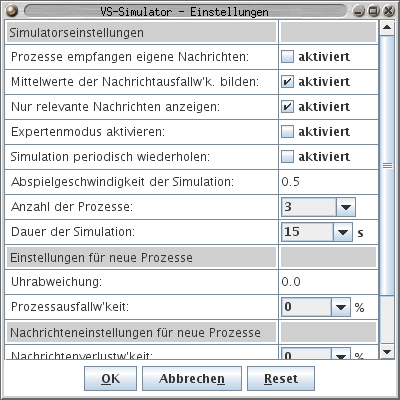
\includegraphics{images/ss-simulationseinstellungen}}
	%\fbox{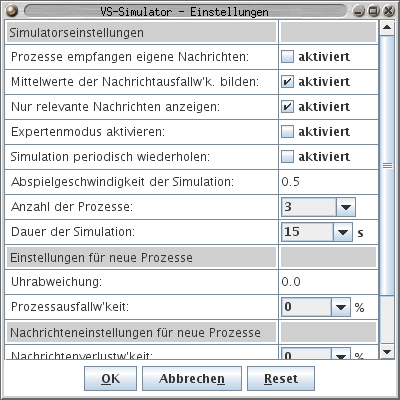
\includegraphics[width=11cm]{images/ss-simulationseinstellungen}}
	\caption{Das Fenster zu den Simulationseinstellungen}
	\label{fig:Simulationseinstellungen}
\end{figure}


Der Simulator unterscheidet zwischen mehreren Datentypen, in denen die einstellbaren Variablen vorliegen k\"{o}nnen (Tabelle \ref{tb:VariablenDatentypen}). Im folgenden bedeutet \texttt{Prefix}: \textit{wert}, dass die Variable vom Typ \texttt{Prefix} ist, und standardm\"{a}ssig den Wert \textit{wert} zugewiesen hat. Vom Anwender lassen sich lediglich die Variablenwerte, jedoch nicht die Variablentypen sowie Variablennamen, \"{a}ndern.

\subsection{Simulationseinstellungen}

\begin{figure}[htbp]
	\centering
	\fbox{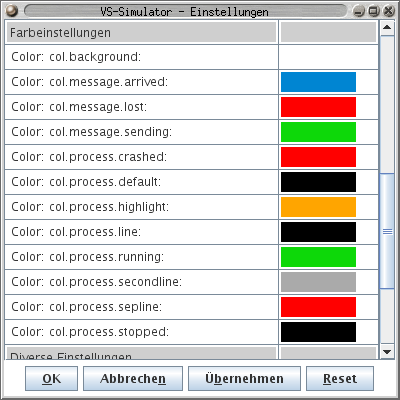
\includegraphics{images/ss-simulationseinstellungen-experten}}
	\caption{Weitere Simulationseinstellungen im Expertenmodus}
	\label{fig:SimulationseinstellungenExperten}
\end{figure}


Beim Erstellen einer neuen Simulation erscheint zun\"{a}chst das dazugeh\"{o}rige Einstellungsfenster (Abbildung \ref{fig:Simulationseinstellungen}). In der Regel reicht es, wenn der Anwender hier die Standardwerte \"{u}bernimmt. Es besteht auch die M\"{o}glichkeit die Einstellungen nachtr\"{a}glich zu editieren, indem das Einstellungsfenster via ``Editieren $\rightarrow$ Einstellungen'' erneut aufgerufen wird.

Im Folgenden werden alle in den Simulationseinstellungen verf\"{u}gbaren Variablen beschrieben. Die Klammern geben den Typen und die Standardwerte an, in denen die Variablen vorliegen. 

\begin{itemize}
	\item \textbf{Prozesse empfangen eigene Nachrichten} \textit{(Boolean: false)}: Standardm\"{a}�ig k\"{o}nnen Prozesse \"{u}bersichtshalber keine Nachrichten empfangen, die sie selbst verschickt haben. Wenn diese Variable jedoch auf \texttt{true} gesetzt wird, dann kann ein Prozess auch selbst verschickte Nachrichten emfpangen und auf diese ebenso antworten. Die Zeit f\"{u}r das Versenden und Empfangen einer Nachricht an sich selbst betr\"{a}gt jedoch stets \texttt{0ms}. Diese Variable sollte mit Vorsicht verwendet werden, da hierdurch, bedingt aus den \texttt{0ms}, Endlosschleifen entstehen k\"{o}nnen. 
	\item \textbf{Mittelwerte der Nachrichtenverlustwahrscheinlichkeiten bilden} \textit{(Boolean, true)}: Jede Nachricht die verschickt wird hat, je nach Einstellungen, eine vom verschickendem Prozess abh\"{a}ngige zuf\"{a}llige \"{U}bertragungszeit bis sie ihr Ziel erreicht. Wenn diese Option aktiviert ist, so wird der Mittelwert vom Sende- und Empfangsprozess gebildet. Ansonsten wird stets die \"{U}bertragungszeit, die beim Senderprozesses angegeben wurde, verwendet.
	\item \textbf{Nur relevante Nachrichten anzeigen} \textit{(Boolean: true)}: Wenn nur alle relevanten Nachrichten angezeigt werden, so werden Nachrichten an einen Prozess die er selbst nicht verarbeiten kann, weil er das dazugeh\"{o}rige Protokoll nicht unterst\"{u}tzt, nicht angezeigt. Hierdurch wird eine Simulation viel \"{u}bersichtlicher dargestellt.
	\item \textbf{Expertenmodus aktivieren} \textit{(Boolean, false)}: Hier l\"{a}sst sich der Expertenmodus auf einen alternativen Weg aktivieren beziehungsweise wieder deaktivieren. 
	\item \textbf{Simulation periodisch wiederholen} \textit{(Boolean: false)}: Wenn diese Variable auf \texttt{true} gesetzt ist, so wird die Simulation jedes Mal nach Ablauf automatisch erneut gestartet. 
	\item \textbf{Abspielgeschwindigkeit der Simulation} \textit{(Float: 0.5)}: Gibt den Faktor der Simulationsabspielgeschindigkeit an. Wenn als Faktor \texttt{1} gew\"{a}hlt wird, dann dauert eine simulierte Sekunde so lange wie eine echte Sekunde. Der Faktor \texttt{0.5} gibt somit an, dass die Simulation mit halber Echtzeitgschwindigkeit abgespielt wird.
	\item \textbf{Anzahl der Prozesse} \textit{(Integer: 3)}: Gibt an wieviele Prozesse an der Simulation teilnehmen sollen. Wie schon erw\"{a}hnt kann der Anwender auch nachtr\"{a}glich via Rechtsklick auf den Prozessbalken den jeweiligen Prozess aus der Simulation entfernen oder weitere Prozesse hinzuf\"{u}gen.
	\item \textbf{Dauer der Simulation} \textit{(Integer: 15)}: Gibt die Dauer der Simulation in Sekunden an.
\end{itemize}

Die weiteren Einstellungen unter ``Einstellungen f\"{u}r neue Prozesse'' sowie ``Nachrichteneinstellungen f\"{u}r neue Prozesse'' geben lediglich Standardwerte an, die f\"{u}r neu zu erstellende Prozesse verwendet werden. Die dort verf\"{u}gbaren Variablen werden im folgenden Teilkapitel genauer beschrieben.

\subsection{Prozess- und Protokolleinstellungen}

Jeder Prozess besitzt folgende Variablen, die entweder via dem Variablen-Tab in der Sidebar oder ``Editieren $\rightarrow$ Prozess \textit{PID}'' oder Linksklick auf den Prozessbalken editiert werden k\"{o}nnen. Das Fenster f\"{u}r die Prozesseinstellungen wird auch als Prozesseditor bezeichnet.

\begin{itemize}
	\item \textbf{Uhrabweichung} \textit{(Float: 0.0)}: Gibt den Faktor an, um den die lokale Prozessuhr abweicht. Der Faktor \texttt{0.0} besagt beispielsweise, dass die Uhr keine Abweichung hat. Ein Faktor von \texttt{1} w\"{u}rde hingegen bedeuten, dass die Uhr mit doppelter Geschwindigkeit liefe. Sind sind nur Werte > \texttt{-1.0} erlaubt, da sonst die Prozessuhr r\"{u}ckw\"{a}rts laufen k\"{o}nnte. Bei allen anderen Werten wird der Faktor wieder automatisch auf \texttt{0.0} gesetzt. Da der Simulator intern mit Flie�kommazahlen doppelter Genauigkeit arbeitet, kann es zu kleinen, jedoch vernachl\"{a}ssigbaren, Rundungsfehlern kommen. 
	\item \textbf{Prozessausfallwahrscheinlichkeit} \textit{(Integer: 0)}: Gibt eine Wahrscheinlichkeit in Prozent an, ob der gegebene Prozess w\"{a}hrend der Simulation zuf\"{a}llig abst\"{u}rzt. Die Wahrscheinlichkeit bezieht sich auf die komplette Simulationsdauer. Bei einer Einstellung von \texttt{100} Prozent und der Simulationsdauer von \texttt{15} Sekunden st\"{u}rzt der Prozess auf jeden Fall zwischen \texttt{0ms} und \texttt{15000ms} ab. An welcher Stelle dies geschieht wird zuf\"{a}llig bestimmt. Wenn der Prozess nach seinem Absturz wiederbelebt wird, st\"{u}rzt er nicht noch einmal zuf\"{a}llig ab. Dies gilt allerdings nicht, wenn die Prozesseinstellungen nach dem Zufallsabsturz erneut ge\"{a}ndert und \"{u}bernommen wurden, da dann das Zufallsabst\"{u}rzereignis erneut erstellt wurde. 
	\item \textbf{Lokale Zeit} \textit{(Long: 0)}: Gibt die aktuelle lokale Prozesszeit in Millisekunden an. Es empfiehlt sich daher die Simulation, bevor Prozesseinstellungen vorgenommen werden, zu pausieren. 
	\item \textbf{Nachrichtenverlustwahrscheinlichkeit} \textit{(Integer: 0)}: Gibt eine Wahrscheinlichkeit in Prozent an, ob eine vom aktuell ausgew\"{a}hlten Prozess verschickte Nachricht unterwegs verloren geht. An welcher Stelle die Nachricht zwischen dem Sende- und Empfangsprozess verloren geht wird vom Simulator zuf\"{a}llig gew\"{a}hlt.
	\item \textbf{Maximale \"{U}bertragungszeit} \textit{(Long: 2000)}: Gibt die Dauer in Millisekunden an, die eine vom Prozess verschickte Nachricht maximal ben\"{o}tigt, bis sie einen Empf\"{a}ngerprozess erreicht. Im weiteren Verlauf wird dieser Wert mit $t_{max}$ bezeichnet. Der tats\"{a}chlich verwendete Wert wird zuf\"{a}llig zwischen der minimalen- und der maximalen Zeit (jeweils inklusive) gew\"{a}hlt. 
	\item \textbf{Minimale \"{U}bertragungszeit} \textit{(Long: 500)}: Gibt die Dauer in Millisekunden an, die eine vom Prozess verschickte Nachricht minimal ben\"{o}tigt, bis sie einen Empf\"{a}ngerprozess erreicht. Im weiteren Verlauf wird dieser Wert mit $t_{min}$ bezeichnet. Der tats\"{a}chlich verwendete Wert wird zuf\"{a}llig zwischen der minimalen- und der maximalen Zeit (jeweils inklusive) gew\"{a}hlt. \\
		\\
		Wenn die \"{U}bertragungszeit einer Nachricht immer exakt die selbe Zeit in Anspruch nehmen soll, dann m\"{u}ssen die Prozesseinstellungen mit $t_{min} = t_{max}$ konfiguriert werden.

\end{itemize}

Im selben Fenster lassen sich auch die Protokollvariablen editieren. Die Protokollvariablen werden jedoch sp\"{a}ter in der Protokollsektion beschrieben.

\subsection{Einstellungen im Expertenmodus}

\begin{table}
	\centering
	\fbox{
	\begin{tabular}{l|l}
		\textbf{Schl\"{u}ssel} & \textbf{Beschreibung}\\
		\hline 
			\texttt{col.background} & Die Hintergrundfarbe der Simulation\\
			\texttt{col.message.arrived} & Nachrichtenfarbe wenn sie ihr Ziel erreicht hat\\
			\texttt{col.message.lost} & Nachrichtenfarbe wenn sie verloren ging\\
			\texttt{col.message.sending} & Nachrichtenfarbe wenn sie noch unterwegs ist\\
			\textbf{\texttt{col.process.crashed}} & Prozessfarbe wenn er abgest\"{u}rzt ist\\
			\textbf{\texttt{col.process.default}} & Prozessfarbe wenn die Simulation aktuell nicht l\"{a}uft und \\
				& der Prozess aktuell nicht abgest\"{u}rzt ist \\
			\textbf{\texttt{col.process.highlight}} & Prozessfarbe wenn die Maus \"{u}ber seinem Balken liegt\\
			\texttt{col.process.line} & Farbe, in der die kleine ``Prozessfane'' an der auch die \\
				& lokale Prozesszeit angegeben wird, dargestellt wird\\
			\textbf{\texttt{col.process.running}} & Prozessfarbe wenn er nicht abgest\"{u}rzt ist und die\\
				& Simulation aktuell l\"{a}uft\\
			\texttt{col.process.secondline} & Farbe in der die Sekunden-Zeitgitter dargestellt werden \\
			\texttt{col.process.sepline} & Farbe der globalen Zeitachse\\
			\textbf{\texttt{col.process.stopped}} & Prozessfarbe wenn die Simulation pausiert wurde\\
	\end{tabular}
	}
	\caption{Farbeinstellungen}
	\label{tb:Farbeinstellungen}
\end{table}

Im Expertenmodus lassen sich zus\"{a}tzliche Variablen, wie beispielsweise diverse Farbwerte und Anzahl der Pixel verschiedener der GUI-Elemente, editieren. Auf Abbildung \ref{fig:SimulationseinstellungenExperten} sieht der Anwender alle einstellbaren Farben. Die fett-gedruckten Schl\"{u}ssel in Tabelle \ref{tb:Farbeinstellungen} dienen nur als Standardwerte f\"{u}r neuzuerstellenen Prozesse und sind auch jeweils in den Prozesseinstellungen separat editierbar.

\section{Protokolle}

Im Folgenden werden alle verf\"{u}gbaren Protokolle behandelt. Wie bereits beschrieben wird bei Protokollen zwischen Server- und Clientseite unterschieden. Server k\"{o}nnen auf Clientnachrichten, und Client auf Servernachrichten antworten. Jeder Prozess kann beliebig viele Protokolle sowohl Clientseitig als auch Serverseitig untest\"{u}tzen. Theoretisch ist es auch m\"{o}glich, dass ein Prozess f\"{u}r ein bestimmtes Protokoll gleichzeitig Server und Client ist. Der Anwender kann auch weitere eigene Protokolle in der Programmiersprache Java mittels einer speziellen API (Application Programming Interface) erstellen. Wie eigene Protokolle erstellt werden k\"{o}nnen wird sp\"{a}ter behandelt. 

\subsection{Beispiel (Dummy) Protokoll}

Das Dummy-Protokoll dient lediglich als leeres Template f\"{u}r die Erstellung eigener Protokolle. Bei der Verwendung des Dummy-Protokolls werden bei Ereignissen lediglich Loggnachrichten ausgegeben. Es werden aber keine weiteren Aktionen ausgef\"{u}hrt.

\subsection{Das Ping-Pong Protokoll}

\begin{figure}[htbp]
	\centering
	\fbox{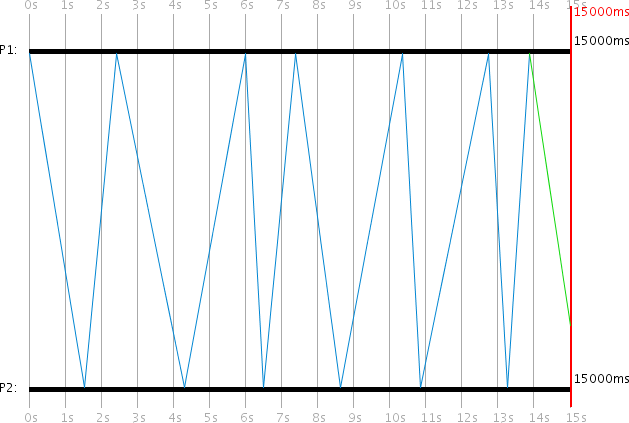
\includegraphics[width=10cm]{images/ss-protokoll-ping-pong}}
	\caption{Das Ping-Pong Protokoll}
	\label{fig:PingPongProto}
\end{figure}

\begin{table}
	\centering
	\fbox{
	\begin{tabular}{c|c|l}
		\textbf{Zeit (ms)} & \textbf{PID} & \textbf{Ereignis} \\
		\hline 
		 	0 & 1 & Ping Pong Client aktivieren\\
		 	0 & 2 & Ping Pong Server aktivieren\\
		 	0 & 1 & Ping Pong Clientanfrage starten
	\end{tabular}
	}
	\caption{Programmierte Ping-Pong Ereignisse}
	\label{tb:PingPongTasks}
\end{table}


Bei dem Ping-Pong Protokoll (Abbildung \ref{fig:PingPongProto}) werden zwischen zwei Prozessen, Client P1 und Server P2, st\"{a}ndig Nachrichten hin- und hergeschickt. Der Ping-Pong Client startet die erste Anfrage, worauf der Server dem Client antwortet. Auf diese Antwort wird vom Client wiederum geantwortet und so weiter. Jeder Nachricht wird ein Z\"{a}hler mitgeschickt, der bei jeder Station um eins inkrementiert- und jeweils im Loggfenster protokolliert wird. In Tabelle \ref{tb:PingPongTasks} sind alle f\"{u}r dieses Beispiel programmierten Ereignisse aufgef\"{u}hrt! Wichtig ist, dass Prozess 1 seinen Ping-Pong Client aktiviert, bevor er eine Ping-Pong Clientanfrage startet! Wenn die Eintrittszeiten f\"{u}r Aktivierung und das Starten der Anfrage identisch sind, so ordnet der Ereigniseditor diese Ereignisse automatisch in der richtigen Reihenfolge an. Wenn der Ping-Pong Client nicht aktiviert werden w\"{u}rde, dann k\"{o}nnte P1 auch keine Ping-Pong Anfrage starten. Der Prozess muss das jeweilige Protokoll unterst\"{u}tzen bevor er eine Anfrage starten kann. Dies gilt nat\"{u}rlich f\"{u}r alle anderen Protokolle analog. Anhand dieses Beispiels ist auch erkennbar, dass die noch nicht ausgelieferte Nachrichten g\"{u}n eingef\"{a}rbt ist. Alle ausgelieferten Nachrichten tragen bereits die Farbe Blau.

\begin{figure}[htbp]
	\centering
	\fbox{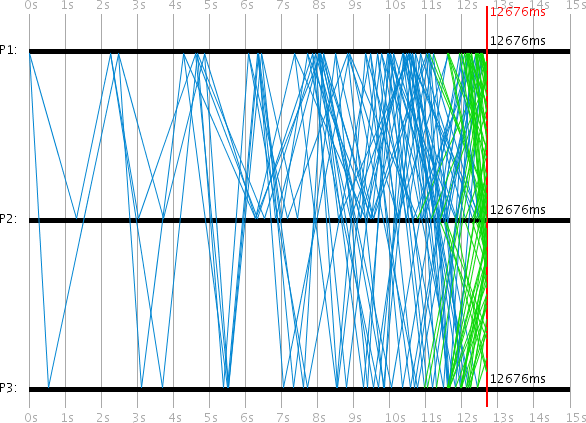
\includegraphics[width=10cm]{images/ss-protokoll-ping-pong-sturm}}
	\caption{Das Ping-Pong Protokoll (Sturm)}
	\label{fig:PingPongSturmProto}
\end{figure}

Werden die Ereignisse wie in Tabelle \ref{tb:PingPongSturmTasks} abge\"{a}ndert, so l\"{a}sst sich ein Ping-Pong Sturm realisieren. Dort wurde ein neuer Prozess 3 eingef\"{u}hrt, der als Ping-Pong Server agiert. Als Resultat verdoppelt sich die Anzahl der kursierenden Nachrichten bei jedem Ping-Pong Durchgang, da auf jede Clientnachricht stets 2 Serverantworten verschickt werden. Auf Abbildung \ref{fig:PingPongSturmProto} ist der dazugeh\"{o}rige Simulationsverlauf dargestellt.

\begin{table}
	\centering
	\fbox{
	\begin{tabular}{c|c|l}
		\textbf{Zeit (ms)} & \textbf{PID} & \textbf{Ereignis} \\
		\hline 
		 	0 & 1 & Ping Pong Client aktivieren\\
		 	0 & 2 & Ping Pong Server aktivieren\\
		 	0 & 3 & Ping Pong Server aktivieren\\
		 	0 & 1 & Ping Pong Clientanfrage starten
	\end{tabular}
	}
	\caption{Programmierte Ping-Pong Ereignisse (Sturm)}
	\label{tb:PingPongSturmTasks}
\end{table}

\subsection{Das Broadcast-Sturm Protokoll}

\begin{figure}[htbp]
	\centering
	\fbox{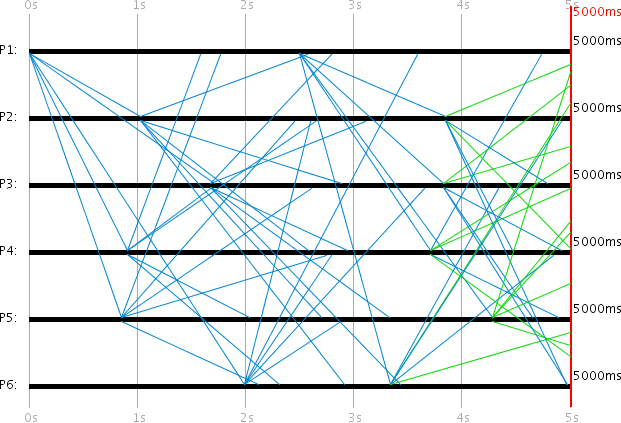
\includegraphics[width=10cm]{images/ss-protokoll-broadcast-sturm}}
	\caption{Das Broadcast-Sturm Protokoll}
	\label{fig:BroadcastSturmProto}
\end{figure}

Das Broadcast-Sturm Protokoll verh\"{a}lt sich \"{a}hnlich wie das Ping-Pong Protokoll. Der Unterschied besteht darin, dass sich das Protokoll anhand einer eindeutigen Broadcast-ID merkt, welche Nachrichten bereits verschickt wurden. Das Broadcast-Sturm Protokoll (Server- und Clientseitig) verschickt alle erhaltenen Nachrichten, sofern sie vom jeweiligen Prozess noch nicht schon einmal verschickt wurden, erneut. Somit l\"{a}sst sich, unter Verwendung mehrerer Prozesse (hier 6), wie auf Abbildung \ref{fig:BroadcastSturmProto}, ein Broadcast-Sturm erzeugen. P1 ist der Client und startet je eine Anfrage nach \texttt{0ms} und \texttt{2500ms}. Die Simulationsdauer betr\"{a}gt hier genau \texttt{5000ms}. Da Client nur Servernachrichten und Server nur Clientnachrichten empfangen k\"{o}nnen, ist in dieser Simulation jeder Prozess, wie in Tabelle \ref{tb:BroadcastSturmTasks} angegeben, gleichzeitig Server und Client. 

\begin{table}
	\centering
	\fbox{
	\begin{tabular}{c|c|l}
		\textbf{Zeit (ms)} & \textbf{PID} & \textbf{Ereignis} \\
		\hline 
		 	0000 & 1 & Broadcaststurn Client aktivieren\\
		 	0000 & 2 & Broadcaststurn Client aktivieren\\
		 	0000 & 3 & Broadcaststurn Client aktivieren\\
		 	0000 & 4 & Broadcaststurn Client aktivieren\\
		 	0000 & 5 & Broadcaststurn Client aktivieren\\
		 	0000 & 6 & Broadcaststurn Client aktivieren\\
		 	0000 & 1 & Broadcaststurn Server aktivieren\\
		 	0000 & 2 & Broadcaststurn Server aktivieren\\
		 	0000 & 3 & Broadcaststurn Server aktivieren\\
		 	0000 & 4 & Broadcaststurn Server aktivieren\\
		 	0000 & 5 & Broadcaststurn Server aktivieren\\
		 	0000 & 6 & Broadcaststurn Server aktivieren\\
		 	0000 & 1 & Broadcaststurn Clientanfrage starten\\
		 	2500 & 1 & Broadcaststurn Clientanfrage starten
	\end{tabular}
	}
	\caption{Programmierte Broadcast-Sturm Ereignisse}
	\label{tb:BroadcastSturmTasks}
\end{table}

\subsection{Das Protokoll zur internen Synchronisierung in einem synchronen System}

\begin{figure}[htbp]
	\centering
	\fbox{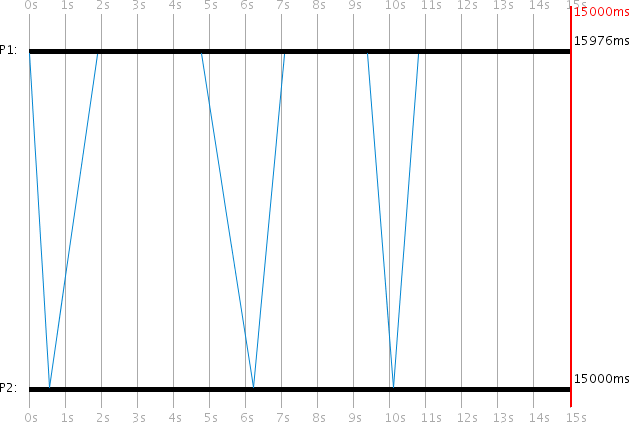
\includegraphics[width=10cm]{images/ss-protokoll-time-sync}}
	\caption{Das Protokoll zur internen Synchronisierung}
	\label{fig:TimeSyncProto}
\end{figure}

Bisher haben wir uns nur mit Protokollen besch\"{a}ftigt, in denen die beteiligten Prozesse keine Uhrabweichung hatten. Das Protokoll zur internen Synchronisierung ist ein Protokoll zur Synchronisierung der lokalen Prozesszeit, welches beispielsweise angewandt werden kann, wenn eine Prozesszeit aufgrund einer Uhrabweichung falsch geht. Wenn der Client seine falsche lokale Zeit $t_c$ mit einem Server synchronisieren m\"{o}chte, so schickt er ihm eine Clientanfrage. Der Server schickt als Antwort seine eigene lokale Prozesszeit $t_s$ zur\"{u}ck, womit der Client seine neue und genauere Prozesszeit berechnen kann. Wie genau die neue Prozesszeit berechnet wird, wird im Folgenden beschrieben. 

\begin{table}
	\centering
	\fbox{
	\begin{tabular}{c|c|l}
		\textbf{Zeit (ms)} & \textbf{PID} & \textbf{Ereignis} \\
		\hline 
		 	00000 & 1 & Interne Sync. Client aktivieren \\
		 	00000 & 2 & Interne Sync. Server aktivieren\\
		 	00000 & 1 & Interne Sync. Clientanfrage starten\\
		 	05000 & 1 & Interne Sync. Clientanfrage starten\\
		 	10000 & 1 & Interne Sync. Clientanfrage starten\\
	\end{tabular}
	}
	\caption{Programmierte Ereignisse zur internen Synchronisierung}
	\label{tb:InterneSyncTasks}
\end{table}

Hier (Abbildung \ref{fig:TimeSyncProto}) stellt P1 den Client und P2 den Server dar. Da die \"{U}bertragungszeit $t_u$ einer Nachricht angenommen zwischen $t'_{min}$ und $t'_{max}$ liegt, setzt der Client P1 nach Empfang der Serverantwort seine lokale Prozesszeit auf 

\begin{equation*}
	t_c := t_s + \frac{1}{2} (t'_{min} + t'_{max})
\end{equation*}

Somit wurde die lokale Zeit von P1, bis auf einen Fehler von $< \frac{1}{2} (t'_{max} - t'_{min})$, synchronisiert. 

Der Clientprozess hat in der Abbildung \ref{fig:TimeSyncProto} als Uhrabweichung den Wert \texttt{0.1} und der Server hat als Uhrabweichung den Wert \texttt{0.0} konfiguriert. Der Client startet, wie in Tabelle \ref{tb:InterneSyncTasks} angegeben, nach \texttt{0ms}, \texttt{5000ms} und \texttt{10000ms} seiner lokalen Prozesszeit jeweils eine Clientanfrage. In der Abbildung l\"{a}sst sich erkennen, dass die 2. und die 3. Anfrage nicht synchron zu der globalen Zeit (Sekunden-Gatter) gestartet werden, was auf die Uhrabweichung von P1 zur\"{u}ckzuf\"{u}hren ist. Nach Simulationsende ist die Zeit von P1 bis auf \texttt{15000ms} - \texttt{15976ms} = \texttt{-976ms} synchronisiert.

\subsubsection{Protokollvariablen}

Dieses Protokoll verwendet folgende zwei clientseitige Variablen, die in den Prozesseinstellungen unter dem Punkt ``Interne Sync. Client'' konfiguriert werden k\"{o}nnen. Serverseitig gibt es hier keine Variablen.

\begin{itemize}
	\item \textbf{Min. \"{U}bertragungszeit} \textit{(Long: 500)}: Gibt den Wert $t'_{min}$ in Millisekunden an
	\item \textbf{Max. \"{U}bertragungszeit} \textit{(Long: 2000)}: Gibt den Wert $t'_{max}$ in Millisekunden an
\end{itemize}

$t'_{min}$ und $t'_{max}$ sind die bei den Protokollberechnungen verwendeten Werte. Sie k\"{o}nnen sich allerdings von den tats\"{a}chlichen Nachrichten\"{u}bertragungszeiten $t_{min}$ und $t_{max}$ (siehe Sektion \"{u}ber Prozesseinstellungen) abweichen. Somit lassen sich auch Szenarien simulieren, in denen das Protokoll falsch eingestellt wurde und in der Zeitsynchronisation gr\"{o}ssere Fehler auftreten k\"{o}nnen.

\subsection{Christians Methode zur externen Synchronisierung}

\begin{figure}[htbp]
	\centering
	\fbox{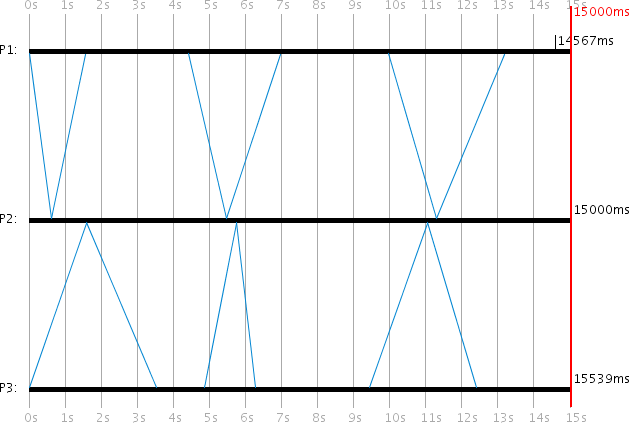
\includegraphics[width=10cm]{images/ss-protokoll-time-sync-2}}
	\caption{Interne Synchronisierung und Christians Methode im Vergleich}
	\label{fig:TimeSync2Proto}
\end{figure}

Ein weiteres Protokoll f\"{u}r die Synchronisierung von Uhrzeiten funktioniert nach der Christians Methode zur externen Synchronisierung. Die Christians Methode benutzt die RTT (Round Trip Time) $t_{rtt}$, um die \"{U}bertragungszeiten von einzelnen Nachrichten zu approximieren. 

Wenn der Client seine lokale Zeit $t_c$ bei einem Server synchronisieren m\"{o}chte, so verschickt er eine Anfrage, und misst dabei bis zur Ankunft der Serverantwort die dazugeh\"{o}rige RTT $t_{rtt}$. Die Serverantwort beinhaltet die lokale Prozesszeit vom Server $t_s$ von dem Zeitpunkt, als der Server die Antwort verschickte. Der Client setzt dann seine lokale Zeit neu mit

\begin{equation*}
	t_c := t_s + \frac{1}{2} t_{rtt}
\end{equation*}

und zwar mit einer Genauigkeit von $\pm(\frac{1}{2} t_{rtt} - u_{min}$) wenn $u_{min}$ eine Schranke f\"{u}r eine Nachrichten\"{u}bertragung mit $t_{rtt} < u_{min}$ ist (siehe \cite{Vorlesung}).

Im Prinzip sieht eine Christians-Simulation so aus wie auf Abbildung \ref{fig:TimeSyncProto}, daher wird hier auf eine einfache Abbildung vom Christians-Protokoll verzichtet. Viel Interessanter ist der direkte Vergleich zwischen dem Protokoll zur internen Synchronisierung und der Christians Methode der externen Synchronisierung (Abbildung \ref{fig:TimeSync2Proto}). Hier stellt P1 den Client zur internen Synchronisierung und P3 den Client zur externen Synchronisierung dar. P2 fungiert f\"{u}r beide Protokolle gleichzeitig als Server. P1 und P3 starten jeweils zu den lokalen Prozesszeiten \texttt{0ms}, \texttt{5000ms} und \texttt{10000ms} eine Clientanfrage (Tabelle \ref{tb:InterneSync2Tasks}). P1 und P3 haben als Uhrabweichung \texttt{0.1} eingestellt und die Simulationsdauer betr\"{a}gt insgesamt \texttt{15000ms}.

Es ist auf Abbildung \ref{fig:TimeSync2Proto} ablesbar, dass nach Ablauf der Simulation P1 seine Zeit bis auf \texttt{15000ms} - \texttt{14567ms} = \texttt{433ms} und P3 seine Zeit bis auf \texttt{15000ms} - \texttt{15539ms} = \texttt{-539ms} synchronisiert hat. In diesem Beispiel hat also das Protokoll zur internen Synchronisierung ein besseres Ergebnis geliefert. Dies ist allerdings nicht zwingend immer der Fall, da nach einer erneuten Ausf\"{u}hrung alle Nachrichten jeweils eine neue zuf\"{a}llige \"{U}bertragungszeit zwischen $t_{min}$ und $t_{max}$ haben werden, die auf das eine oder andere Protokoll wieder andere Auswirkungen haben k\"{o}nnen.

\begin{table}
	\centering
	\fbox{
	\begin{tabular}{c|c|l}
		\textbf{Zeit (ms)} & \textbf{PID} & \textbf{Ereignis} \\
		\hline 
		 	00000 & 1 & Interne Sync. Client aktivieren \\
		 	00000 & 1 & Interne Sync. Clientanfrage starten\\
		 	00000 & 2 & Christians Server aktivieren\\
		 	00000 & 2 & Interne Sync. Server aktivieren\\
		 	00000 & 3 & Christians Client aktivieren \\
		 	00000 & 3 & Christians Clientanfrage starten\\
		 	05000 & 1 & Interne Sync. Clientanfrage starten\\
		 	05000 & 3 & Christians Clientanfrage starten\\
		 	10000 & 1 & Interne Sync. Clientanfrage starten\\
		 	10000 & 3 & Christians Clientanfrage starten\\
	\end{tabular}
	}
	\caption{Programmierte Ereignisse, Vergleich interne und externe Synchronisierung}
	\label{tb:InterneSync2Tasks}
\end{table}

\subsection{Der Berkeley Algorithmus zur internen Synchronisierung}

\begin{figure}[htbp]
	\centering
	\fbox{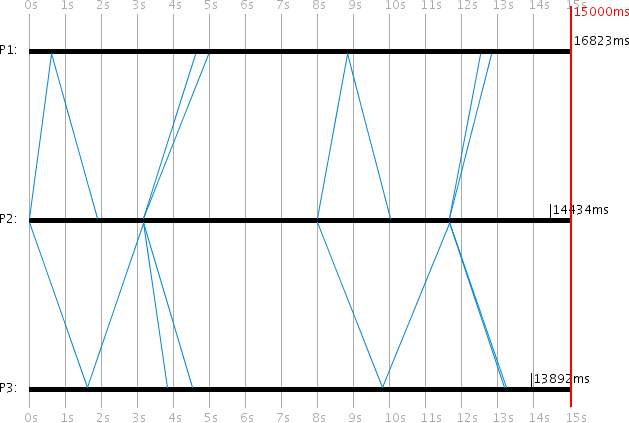
\includegraphics[width=10cm]{images/ss-protokoll-berkeley}}
	\caption{Der Berkeley Algorithmus zur internen Synchronisierung}
	\label{fig:BerkeleyProto}
\end{figure}

Der Berkeley Algorithmus zur internen Synchronisierung ist eine weitere M\"{o}glichkeit lokale Uhrzeiten abzugleichen. Dies ist das erste Protokoll, bei dem der Server die initiale Anfrage startet. Der Server stellt den Koordinator des Protokolls dar. Die Clients sind somit passiv und m\"{u}ssen warten, bis eine Serveranfrage eintritt. Hierbei muss der Server wissen, welche Clientprozesse an dem Protokoll teilnehmen, was sich in den Prozesseinstellungen des Servers einstellen l\"{a}sst.

\begin{table}
	\centering
	\fbox{
	\begin{tabular}{c|c|l}
		\textbf{Zeit (ms)} & \textbf{PID} & \textbf{Ereignis} \\
		\hline 
		 	0000 & 1 & Berkeley Client aktivieren \\
		 	0000 & 2 & Berkeley Server aktivieren \\
		 	0000 & 3 & Berkeley Client aktivieren \\
		 	0000 & 2 & Berkeley Serveranfrage starten\\
		 	7500 & 2 & Berkeley Serveranfrage starten\\
	\end{tabular}
	}
	\caption{Programmierte Ereignisse zum Berkeley Algorithmus}
	\label{tb:BerkeleyTasks}
\end{table}

Wenn der Server seine eigene lokale Zeit $t_s$ und auch die lokalen Prozesszeiten $t_i$ der Clients ($i = 1, ..., n$) synchronisieren m\"{o}chte, so verschickt er eine Serveranfrage. $n$ sei hierbei die Anzahl beteiligter Clients. Die Clients senden dann ihre lokalen Prozesszeiten in einer Nachricht zur\"{u}ck zum Server. Der Server hat dabei die RTTs $r_i$ bis zur Ankunft aller Clientantworten gemessen. 

Nachdem alle Antworten vorliegen, setzt er zun\"{a}chst seine eigene Zeit $t_s$ auf den Mittelwert $t_{avg}$ aller bekannten Prozesszeiten (seiner eigenen Prozesszeit eingeschlossen). Die \"{U}bertragungszeit einer Clientantwort wird auf die h\"{a}lfte der RTT gesch\"{a}tzt und wird in der Berechnung ber\"{u}cksichtigt. 

\begin{equation*}
	t_{avg} :=
	\frac{1}{n+1} ( t_s +
		\sum_{\substack{
			i=1\\
		}}^n
		\frac{r_i}{2} + t_i
	)
\end{equation*}
\begin{equation*}
	t_s := t_{avg}
\end{equation*}

Anschlie�end berechnet der Server f\"{u}r jeden Client einen Korrekturwert $k_i := t_{avg} - t_i$, den er jeweils in einer separaten Nachricht zur\"{u}ckschickt. Die Clients setzten dann jeweils die lokale Prozesszeit auf $t'_i := t'_i + k_i$. Hierbei stellt $t'_i$ die derzeit aktuelle Prozesszeit des jeweiligen Clients dar. Denn bis zum Eintreffen des Korrekturwertes ist inzwischen wieder Zeit verstrichen.

In den Beispiel auf Abbildung \ref{fig:BerkeleyProto} gibt es 2 Clientprozesse P1 und P3 sowie den Serverprozess P2. Der Server startet nach jeweils \texttt{0ms} und \texttt{7500ms} eine Synchronisationsanfrage (Tabelle \ref{tb:BerkeleyTasks}). In dieser Abbildung ist erkennbar, dass der Server stets 2 Korrekturwerte verschickt, die jeweils P1 und P2 erreichen. Es werden hier also pro Synchronisierungsvorgang 4 Korrekturwerte ausgeliefert. Eine Korrekturnachricht enth\"{a}lt neben dem Korrekturwert $k_i$ auch die PID des Prozesses, f\"{u}r den die Nachricht bestimmt ist. Ein Client verarbeiten so nur die f\"{u}r ihn bestimmten Korrekturwerte, indem das Protokoll die PID vorher \"{u}berpr\"{u}ft. 

\subsubsection{Protokollvariablen}

Dieses Protokoll verwendet folgende serverseitige Variable, die in den Prozesseinstellungen unter dem Punkt ``Berkeley Server'' konfiguriert werden kann. Clientseitig gibt es hier keine Variablen.

\begin{itemize}
	\item \textbf{PIDs beteiliger Prozesse} \textit{(Integer[]: [1,3])}: Dieser Vektor aus Integerwerten beinhaltet alle PIDs der Berkeley Clientprozesse, mit denen der Berkeley Server die Zeit synchronisieren soll. Das Protokoll funktioniert nicht wenn hier eine PID angegeben wird die gar nicht existiert oder nicht das Berkeley Protokoll clientseitig unterst\"{u}tz. In diesem Fall w\"{u}rde ewig auf eine fehlende Clientantwort gewartet werden.
\end{itemize}

\subsection{Das Ein-Phasen Commit Protokoll}

\begin{figure}[htbp]
	\centering
	\fbox{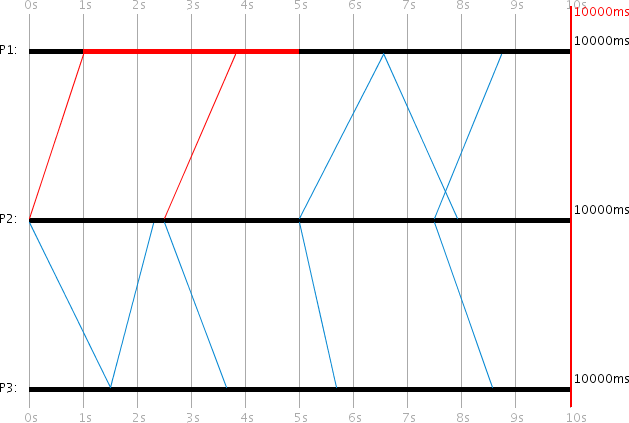
\includegraphics[width=10cm]{images/ss-protokoll-one-phase-commit}}
	\caption{Das Ein-Phasen Commit Protokoll}
	\label{fig:OnePhaseCommitProto}
\end{figure}

Das Ein-Phasen Commit Protokoll ist daf\"{u}r da, beliebig vielen Clients zu einer Festschreibung zu bewegen. Im realen Leben k\"{o}nnte dies beispielsweise das Erstellen oder L\"{o}schen einer Datei sein, von der auf jedem Client eine lokale Kopie existiert. Der Server ist der Koordinator und auch derjenige, der einen Festschreibewunsch initiiert. Hierbei verschickt der Server periodisch so oft den Festschreibewunsch, bis er von jedem Client eine Best\"{a}tigung erhalten hat. Der Server muss dabei die PIDs aller beteiligten Clientprozesse sowie einen Wecker f\"{u}r erneutes Versenden des Festschreibewunsches eingestellt bekommen. 

Die programmierten Ereignisse des Beispiels auf Abbildung \ref{fig:OnePhaseCommitProto} sind in Tabelle \ref{tb:OnePhaseCommitTasks} aufgelistet. P1 und P3 simulieren jeweils einen Client und P2 den Server. Damit die Simulation mehrere Festschreibew\"{u}nsche verschickt, st\"{u}rzt in der Simulation P1 nach \texttt{1000ms} ab und nach \texttt{5000ms} steht er wieder zur Verf\"{u}gung. Die ersten beide Festschreibew\"{u}nsche erreichen dadurch P1 nicht und erst der dritte Versuch verl\"{a}uft erfolgreich. Bevor die Best\"{a}tigung von P1 bei P2 eintrifft, l\"{a}uft jedoch der Wecker erneut ab, so dass ein weiterer Festschreibewunsch versendet wird. Da P1 und P3 jeweils schon eine Best\"{a}tigung verschickt haben, wird diese Nachricht zum Festschreibewunsch ignoriert. 

\begin{table}
	\centering
	\fbox{
	\begin{tabular}{c|c|l}
		\textbf{Zeit (ms)} & \textbf{PID} & \textbf{Ereignis} \\
		\hline 
		 	0000 & 1 & 1-Phasen Commit Client aktivieren\\
		 	0000 & 2 & 1-Phasen Commit Server aktivieren\\
		 	0000 & 3 & 1-Phasen Commit Client aktivieren\\
		 	0000 & 2 & 1-Phasen Commit Serveranfrage starten\\
		 	1000 & 1 & Prozessabsturz\\
		 	5000 & 1 & Prozesswiederbelebung
	\end{tabular}
	}
	\caption{Programmierte Ein-Phasen Commit Ereignisse}
	\label{tb:OnePhaseCommitTasks}
\end{table}

\subsubsection{Protokollvariablen}

Dieses Protokoll verwendet folgende serverseitige Variablen, die in den Prozesseinstellungen unter dem Punkt ``1-Phasen Commit Server'' konfiguriert werden k\"{o}nnen. Clientseitig gibt es hier keine Variablen.

\begin{itemize}
	\item \textbf{Zeit bis erneute Anfrage} \textit{(Long: 2500)}: Gibt die Anzahl von Millisekunden an, die gewartet werden sollen, bis der Festschreibewunsch erneut verschickt wird.
	\item \textbf{PIDs beteiliger Prozesse} \textit{(Integer[]: [1,3])}: Dieser Vektor aus Integerwerten beinhaltet alle PIDs der Clientprozesse, die festschreiben sollen. 
\end{itemize}

\subsection{Das Zwei-Phasen Commit Protokoll}

\begin{figure}[htbp]
	\centering
	\fbox{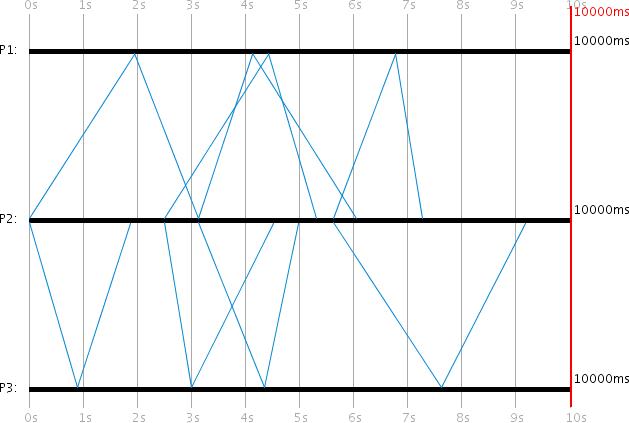
\includegraphics[width=10cm]{images/ss-protokoll-two-phase-commit}}
	\caption{Das Zwei-Phasen Commit Protokoll}
	\label{fig:TwoPhaseCommitProto}
\end{figure}

Das Zwei-Phasen Commit Protokoll ist eine Erweiterung des Ein-Phasen Commit Protokolls. Der Server startet zun\"{a}chst eine Anfrage an alle beteiligten Clients, ob festgeschrieben werden soll. Jeder Client antwortet dann mit \texttt{true} oder \texttt{false}. Der Server fragt so oft periodisch nach, bis ein Ergebnis aller Clients vorliegt. Nach Erhalt aller Abstimmungen \"{u}berpr\"{u}ft der Server, ob alle mit \texttt{true} abgestimmt haben. F\"{u}r den Fall dass mindestens ein Client mit \texttt{false} abgestimmt hat, wird der Festschreibevorgang abgebrochen und als globales Abstimmungsergebnis \texttt{false} verschickt. Wenn alle jedoch mit \texttt{true} abstimmten, soll festgeschrieben werden. Dabei wird das globale Abstimmungsergebnis \texttt{true} verschickt. Das globale Abstimmungsergebnis wird periodisch so oft erneut verschickt, bis von jedem Client eine Best\"{a}tigung des Erhalts vorliegt.

\begin{table}
	\centering
	\fbox{
	\begin{tabular}{c|c|l}
		\textbf{Zeit (ms)} & \textbf{PID} & \textbf{Ereignis} \\
		\hline 
		 	0000 & 1 & 2-Phasen Commit Client aktivieren\\
		 	0000 & 2 & 2-Phasen Commit Server aktivieren\\
		 	0000 & 3 & 2-Phasen Commit Client aktivieren\\
		 	0000 & 2 & 2-Phasen Commit Serveranfrage starten
	\end{tabular}
	}
	\caption{Programmierte Zwei-Phasen Commit Ereignisse}
	\label{tb:TwoPhaseCommitTasks}
\end{table}

In dem Beispiel (Abbildung \ref{fig:TwoPhaseCommitProto}) sind P1 und P3 Clients und P2 der Server. Der Server verschickt nach \texttt{0ms} seine initiale Anfrage (Tabelle \ref{tb:TwoPhaseCommitTasks}). Da diese Simulation recht un\"{u}bersichtlich ist, liegen in den Tabellen \ref{tb:TwoPhaseCommitLoggs} und \ref{tb:TwoPhaseCommitLoggs2} Ausz\"{u}ge aus dem Loggfenster vor. Auf die Lamport- und Vektorzeitstempel sowie die lokalen Prozesszeiten wurde hier wegen Irrelevanz verzichtet. Da keine Uhrabweichungen konfiguriert wurden, sind die lokalen Prozesszeiten stets gleich der globalen Zeit und deswegen wird hier pro Loggeintrag jeweils nur eine Zeit angegeben. Anhand der Nachrichten IDs lassen sich dort die einzelnen Sendungen zuordnen. Hier stimmen P1 und P3 jeweils mit \texttt{true}, d.h. es soll festgeschrieben werden, ab. In den Loggs wird auch st\"{a}ndig der Inhalt der verschickten Nachricht sowie die dazugeh\"{o}rigen Datentypen aufgef\"{u}hrt.

\begin{table}
	\centering
	\fbox{
	\begin{tabular}{c|c|l}
		\textbf{Zeit (ms)} & \textbf{PID} & \textbf{Loggnachricht} \\
			\hline
000000 & & Simulation gestartet\\
\hline
000000 & 1 & 2-Phasen Commit Client aktiviert\\
\hline
000000 & 2 & 2-Phasen Commit Server aktiviert\\
\hline
000000 & 2 & Nachricht versendet; ID: 94; Protokoll: 2-Phasen Commit\\
	& & Boolean: wantVote=true\\
\hline
000000 & 3 & 2-Phasen Commit Client aktiviert\\
\hline
000905 & 3 & Nachricht erhalten; ID: 94; Protokoll: 2-Phasen Commit\\
\hline
000905 & 3 & Nachricht versendet; ID: 95; Protokoll: 2-Phasen Commit\\
	& & Integer: pid=3; Boolean: isVote=true; vote=true\\
\hline
000905 & 3 & Abstimmung true versendet\\
\hline
001880 & 2 & Nachricht erhalten; ID: 95; Protokoll: 2-Phasen Commit\\
\hline
001880 & 2 & Abstimmung von Prozess 3 erhalten! Ergebnis: true\\
\hline
001947 & 1 & Nachricht erhalten; ID: 94; Protokoll: 2-Phasen Commit\\
\hline
001947 & 1 & Nachricht versendet; ID: 96; Protokoll: 2-Phasen Commit\\
	& & Integer: pid=1; Boolean: isVote=true; vote=true\\
\hline
001947 & 1 & Abstimmung true versendet\\
\hline
002500 & 2 & Nachricht versendet; ID: 97; Protokoll: 2-Phasen Commit\\
	& & Boolean: wantVote=true\\
\hline
003006 & 3 & Nachricht erhalten; ID: 97; Protokoll: 2-Phasen Commit\\
\hline
003006 & 3 & Nachricht versendet; ID: 98; Protokoll: 2-Phasen Commit\\
	& & Integer: pid=3; Boolean: isVote=true; vote=true\\
\hline
003006 & 3 & Abstimmung true versendet\\
\hline
003137 & 2 & Nachricht erhalten; ID: 96; Protokoll: 2-Phasen Commit\\
\hline
003137 & 2 & Abstimmung von Prozess 1 erhalten! Ergebnis: true\\
\hline
003137 & 2 & Abstimmungen von allen beteiligten Prozessen erhalten!\\
	& & Globales Ergebnis: true\\
\hline
003137 & 2 & Nachricht versendet; ID: 99; Protokoll: 2-Phasen Commit\\
	& & Boolean: isVoteResult=true; voteResult=true\\
\hline
004124 & 1 & Nachricht erhalten; ID: 99; Protokoll: 2-Phasen Commit\\
\hline
004124 & 1 & Globales Abstimmungsergebnis erhalten. Ergebnis: true\\
\hline
004124 & 1 & Nachricht versendet; ID: 100; Protokoll: 2-Phasen Commit\\
	& & Integer: pid=1; Boolean: isAck=true\\
\hline
004354 & 3 & Nachricht erhalten; ID: 99; Protokoll: 2-Phasen Commit\\
\hline
004354 & 3 & Globales Abstimmungsergebnis erhalten. Ergebnis: true\\
\hline
004354 & 3 & Nachricht versendet; ID: 101; Protokoll: 2-Phasen Commit\\
	& & Integer: pid=3; Boolean: isAck=true\\
\hline
004434 & 1 & Nachricht erhalten; ID: 97; Protokoll: 2-Phasen Commit\\
\hline
004434 & 1 & Nachricht versendet; ID: 102; Protokoll: 2-Phasen Commit\\
	& & Integer: pid=1; Boolean: isVote=true; vote=true\\
	\end{tabular}
	}
	\caption{Auszug aus der Loggausgabe des Zwei-Phasen Commit Beispiels}
	\label{tb:TwoPhaseCommitLoggs}
\end{table}

\begin{table}
	\centering
	\fbox{
	\begin{tabular}{c|c|l}
		\textbf{Zeit (ms)} & \textbf{PID} & \textbf{Loggnachricht} \\
			\hline
004434 & 1 & Abstimmung true versendet\\
\hline
004527 & 2 & Nachricht erhalten; ID: 98; Protokoll: 2-Phasen Commit\\
\hline
004975 & 2 & Nachricht erhalten; ID: 101; Protokoll: 2-Phasen Commit\\
\hline
005311 & 2 & Nachricht erhalten; ID: 102; Protokoll: 2-Phasen Commit\\
\hline
005637 & 2 & Nachricht versendet; ID: 103; Protokoll: 2-Phasen Commit\\
	& & Boolean: isVoteResult=true; voteResult=true\\
\hline
006051 & 2 & Nachricht erhalten; ID: 100; Protokoll: 2-Phasen Commit\\
\hline
006051 & 2 & Alle Teilnehmer haben die Abstimmung erhalten\\
\hline
006766 & 1 & Nachricht erhalten; ID: 103; Protokoll: 2-Phasen Commit\\
\hline
006766 & 1 & Globales Abstimmungsergebnis erhalten. Ergebnis: true\\
\hline
006766 & 1 & Nachricht versendet; ID: 104; Protokoll: 2-Phasen Commit\\
	& & Integer: pid=1; Boolean: isAck=true\\
\hline
007279 & 2 & Nachricht erhalten; ID: 104; Protokoll: 2-Phasen Commit\\
\hline
007618 & 3 & Nachricht erhalten; ID: 103; Protokoll: 2-Phasen Commit\\
\hline
007618 & 3 & Globales Abstimmungsergebnis erhalten. Ergebnis: true\\
\hline
007618 & 3 & Nachricht versendet; ID: 105; Protokoll: 2-Phasen Commit\\
	& & Integer: pid=3; Boolean: isAck=true\\
\hline
009170 & 2 & Nachricht erhalten; ID: 105; Protokoll: 2-Phasen Commit\\
\hline
010000 & & Simulation beendet
	\end{tabular}
	}
	\caption{Auszug aus der Loggausgabe des Zwei-Phasen Commit Beispiels (2)}
	\label{tb:TwoPhaseCommitLoggs2}
\end{table}

\subsubsection{Protokollvariablen}

Dieses Protokoll verwendet folgende serverseitige Variablen, die in den Prozesseinstellungen unter dem Punkt ``2-Phasen Commit Server'' konfiguriert werden k\"{o}nnen:

\begin{itemize}
	\item \textbf{Zeit bis erneute Anfrage} \textit{(Long: 2500)}: Gibt die Anzahl von Millisekunden an, die gewartet werden sollen, bis der Festschreibewunsch erneut verschickt wird.
	\item \textbf{PIDs beteiliger Prozesse} \textit{(Integer[]: [1,3])}: Dieser Vektor aus Integerwerten beinhaltet alle PIDs der Clientprozesse, die \"{u}ber eine Festschreibung abstimmen, und anschlie�end gegebenenfalls festschreiben sollen. 
\end{itemize}

Und folgende Clientvariable kann unter den Prozesseinstellungen unter dem Punkt ``2-Phasen Commit Client'' konfiguriert werden:

\begin{itemize}
	\item \textbf{Festschreibwahrscheinlichkeit} \textit{(Integer: 50)}: Gibt die Wahrscheinlichkeit in Prozent an, die der Client mit \texttt{true}, also f\"{u}r das Festschreiben, abstimmt.
\end{itemize}

\subsection{Der ungen\"{u}gende (Basic) Multicast}

\begin{figure}[htbp]
	\centering
	\fbox{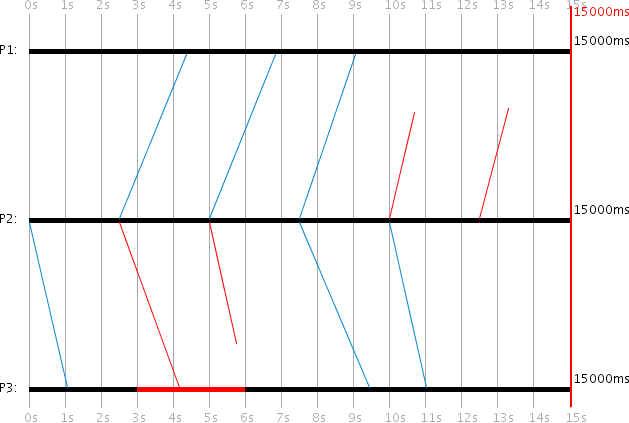
\includegraphics[width=10cm]{images/ss-protokoll-basic-multicast}}
	\caption{Das Basic-Multicast Protokoll}
	\label{fig:BasicMulticastProto}
\end{figure}

\begin{table}
	\centering
	\fbox{
	\begin{tabular}{c|c|l}
		\textbf{Zeit (ms)} & \textbf{PID} & \textbf{Ereignis} \\
		\hline 
		 	00000 & 2 & Basic Multicast Client aktivieren\\
		 	00000 & 3 & Basic Multicast Server aktivieren\\
		 	00000 & 2 & Basic Multicast Clientanfrage starten\\
		 	02500 & 1 & Basic Multicast Server aktivieren\\
		 	02500 & 2 & Basic Multicast Clientanfrage starten\\
		 	03000 & 3 & Prozessabsturz\\
		 	05000 & 2 & Basic Multicast Clientanfrage starten\\
		 	06000 & 3 & Prozesswiederbelebung\\
		 	07500 & 2 & Basic Multicast Clientanfrage starten\\
		 	10000 & 2 & Basic Multicast Clientanfrage starten\\
		 	12500 & 2 & Basic Multicast Clientanfrage starten
	\end{tabular}
	}
	\caption{Programmierte Basic-Multicast Ereignisse}
	\label{tb:BasicMulticastTasks}
\end{table}


Das Basic-Multicast Protokoll ist sehr einfach aufgebaut. In dem Beispiel auf Abbildung \ref{fig:BasicMulticastProto} sind P1 und P3 Server und P2 der Client. Bei diesem Protokoll startet der Client immer die Anfrage, was bei diesem Protokoll eine einfache Multicast-Nachricht ist, die jeder Server empfangen kann. Wie in Tabelle \ref{tb:BasicMulticastTasks} aufgef\"{u}hrt verschickt P2 alle \texttt{2500ms} jeweils eine Multicast-Nachricht, die alle voneinander v\"{o}llig unabh\"{a}ngig sind. 

P1 kann jedoch erst nach \texttt{2500ms} Multicast-Nachrichten empfangen, da er vorher das Protokoll nicht unterst\"{u}tzt w\"{a}hrend P3 von \texttt{3000ms} bis \texttt{6000ms} abgest\"{u}rzt ist und auch keine Nachrichten empfangen kann. Da die Einstellung ``Nur relevante Nachrichten anzeigen'' aktiviert ist, wird die erste Multicast-Nachricht von P2 an P1 nicht dargestellt. Bei jedem Prozess wurde die Nachrichtenverlustwahrscheinlichkeit auf \texttt{30} Prozent gesetzt, worauf alle in dieser Simulation verschickten Nachrichten mit einer Wahrscheinlichkeit von \texttt{30} Prozent ausfallen. 

In diesem Beispiel ging die 3. Multicast-Nachricht auf den Weg zu P3- und die 5. sowie 6. Nachricht auf den Weg zu P1 verloren. Lediglich die 4. Multicast-Nachricht hat alle Ziele erreicht.

\subsection{Der zuverl\"{a}ssige (Reliable) Multicast}

\begin{figure}[htbp]
	\centering
	\fbox{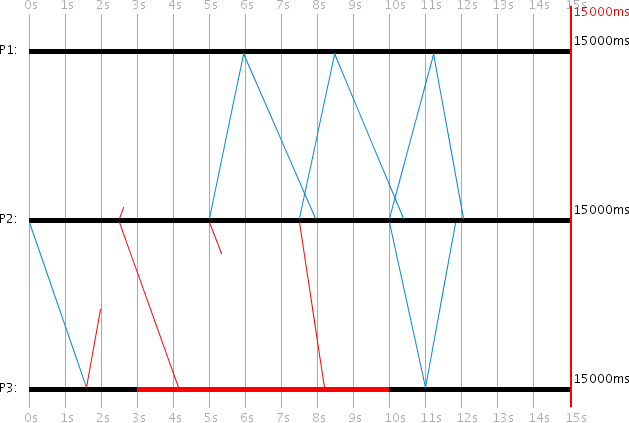
\includegraphics[width=10cm]{images/ss-protokoll-reliable-multicast}}
	\caption{Das Reliable-Multicast Protokoll}
	\label{fig:ReliableMulticastProto}
\end{figure}

Bei dem  zuverl\"{a}ssigen (Reliable) Multicast verschickt der Client so oft periodisch seine Multicast-Nachricht erneut, bis er von allen beteiligten Servern eine Best\"{a}tigung erhalten hat. Nach jedem erneuten Versuch vergisst der Client, von welchen Servern er bereits eine Best\"{a}tigung erhalten hat, womit jeder erneuter Versuch von allen Teilnehmern aufs Neue best\"{a}tigt werden muss. In dem Beispiel (Abbildung \ref{fig:ReliableMulticastProto}, Tabelle \ref{tb:ReliableMulticastTasks}, sowie den Loggs in den Tabellen \ref{tb:ReliableMulticastLoggs} und \ref{tb:ReliableMulticastLoggs2}) ist P2 der Multicast-verschickende Client, w\"{a}hrend P1 und P3 die Server darstellen. Bei \texttt{0ms} initiiert der Client seine Multicast-Nachricht. Die Nachrichtenverlustwahrscheinlichkeiten sind \"{u}berall auf 30 Prozent eingestellt.

In diesem Beispiel ben\"{o}tigt der Client bis zur korrekten Auslieferung des zuverl\"{a}ssigen Multicasts genau 5 Versuche:

\begin{enumerate}
	\setlength{\itemsep}{-2mm}
	\item Versuch: 
		\begin{itemize}
			\setlength{\itemsep}{-2.5mm}
			\item P1 unterst\"{u}tzt das Reliable-Multicast Protokoll noch nicht, und kann somit weder Multicast-Nachricht erhalten noch eine Best\"{a}tigung verschicken.
			\item P3 empf\"{a}ngt die Multicast-Nachricht, jedoch geht seine Best\"{a}tigungsnachricht verloren.
		\end{itemize}
	\item Versuch: 
		\begin{itemize}
			\setlength{\itemsep}{-2.5mm}
			\item P1: Die Multicast-Nachricht geht unterwegs zu P1 verloren.
			\item P3: Die Multicast-Nachricht erreicht P3, aber P3 ist abgest\"{u}rzt und kann somit keine Nachricht verarbeiten.
		\end{itemize}
	\item Versuch: 
		\begin{itemize}
			\setlength{\itemsep}{-2.5mm}
			\item P1 empf\"{a}ngt die Multicast-Nachricht und seine Best\"{a}tigung kommt wie geplant bei P2 an. 
			\item P3: Die Multicast-Nachricht geht unterwegs zu P3 verloren.
		\end{itemize}
	\item Versuch: 
		\begin{itemize}
			\setlength{\itemsep}{-2.5mm}
			\item P1 empf\"{a}ngt die Multicast-Nachricht und seine Best\"{a}tigung kommt wie geplant bei P2 an. 
			\item P3: Die Multicast-Nachricht erreicht P3, aber P3 ist abgest\"{u}rzt und kann somit keine Nachricht verarbeiten.
		\end{itemize}
	\item Versuch: 
		\begin{itemize}
			\item P1 empf\"{a}ngt die Multicast-Nachricht und seine Best\"{a}tigung kommt wie geplant bei P2 an. 
			\setlength{\itemsep}{-2.5mm}
			\item P3 empf\"{a}ngt die Multicast-Nachricht und seine Best\"{a}tigung kommt wie geplant bei P2 an. 
		\end{itemize}
\end{enumerate}

\begin{table}
	\centering
	\fbox{
	\begin{tabular}{c|c|l}
		\textbf{Zeit (ms)} & \textbf{PID} & \textbf{Ereignis} \\
		\hline 
		 	00000 & 3 & Reliable Multicast Server aktivieren\\
		 	00000 & 2 & Reliable Multicast Client aktivieren\\
		 	00000 & 2 & Reliable Multicast Clientanfrage starten\\
		 	02500 & 1 & Reliable Multicast Server aktivieren\\
		 	03000 & 3 & Prozessabsturz\\
		 	10000 & 3 & Prozesswiederbelebung\\
	\end{tabular}
	}
	\caption{Programmierte Reliable-Multicast Ereignisse}
	\label{tb:ReliableMulticastTasks}
\end{table}

\begin{table}
	\centering
	\fbox{
	\begin{tabular}{c|c|l}
		\textbf{Zeit (ms)} & \textbf{PID} & \textbf{Loggnachricht} \\
			\hline
000000 & & Simulation gestartet\\
\hline
000000 & 2 & Reliable Multicast Client aktiviert\\
\hline
000000 & 2 & Nachricht versendet; ID: 280; Protokoll: Reliable Multicast;\\
	   & & Boolean: isMulticast=true\\
\hline
000000 & 3 & Reliable Multicast Server aktiviert\\
\hline
001590 & 3 & Nachricht erhalten; ID: 280; Protokoll: Reliable Multicast\\
\hline
001590 & 3 & Nachricht versendet; ID: 281; Protokoll: Reliable Multicast\\
	   & & Integer: pid=3; Boolean: isAck=true\\
\hline
001590 & 3 & ACK versendet\\
\hline
002500 & 1 & Reliable Multicast Server aktiviert\\
\hline
002500 & 2 & Nachricht versendet; ID: 282; Protokoll: Reliable Multicast\\
	   & & Boolean: isMulticast=true\\
\hline
003000 & 3 & Abgest�rzt\\
\hline
005000 & 2 & Nachricht versendet; ID: 283; Protokoll: Reliable Multicast\\
	   & & Boolean: isMulticast=true\\
\hline
005952 & 1 & Nachricht erhalten; ID: 283; Protokoll: Reliable Multicast\\
\hline
005952 & 1 & Nachricht versendet; ID: 284; Protokoll: Reliable Multicast\\
	   & & Integer: pid=1; Boolean: isAck=true\\
\hline
005952 & 1 & ACK versendet\\
\hline
007500 & 2 & Nachricht versendet; ID: 285; Protokoll: Reliable Multicast\\
	   & & Boolean: isMulticast=true\\
\hline
007937 & 2 & Nachricht erhalten; ID: 284; Protokoll: Reliable Multicast\\
\hline
007937 & 2 & ACK von Prozess 1 erhalten!\\
\hline
008469 & 1 & Nachricht erhalten; ID: 285; Protokoll: Reliable Multicast\\
\hline
008469 & 1 & Nachricht versendet; ID: 286; Protokoll: Reliable Multicast\\
	   & & Integer: pid=1; Boolean: isAck=true\\
\hline
008469 & 1 & ACK erneut versendet\\
\hline
010000 & 2 & Nachricht versendet; ID: 287; Protokoll: Reliable Multicast\\
	   & & Boolean: isMulticast=true\\
\hline
010000 & 3 & Wiederbelebt\\
\hline
010395 & 2 & Nachricht erhalten; ID: 286; Protokoll: Reliable Multicast\\
\hline
010995 & 3 & Nachricht erhalten; ID: 287; Protokoll: Reliable Multicast\\
\hline
010995 & 3 & Nachricht versendet; ID: 288; Protokoll: Reliable Multicast\\
	   & & Integer: pid=3; Boolean: isAck=true\\
\hline
010995 & 3 & ACK erneut versendet\\
\hline
011213 & 1 & Nachricht erhalten; ID: 287; Protokoll: Reliable Multicast\\
\hline
011213 & 1 & Nachricht versendet; ID: 289; Protokoll: Reliable Multicast\\
	   & & Integer: pid=1; Boolean: isAck=true\\
	\end{tabular}
	}
	\caption{Auszug aus der Loggausgabe des Reliable-Multicast Beispiels}
	\label{tb:ReliableMulticastLoggs}
\end{table}

\begin{table}
	\centering
	\fbox{
	\begin{tabular}{c|c|l}
		\textbf{Zeit (ms)} & \textbf{PID} & \textbf{Loggnachricht} \\
			\hline
011213 & 1 & ACK erneut versendet\\
\hline
011813 & 2 &  Nachricht erhalten; ID: 288; Protokoll: Reliable Multicast\\
\hline
011813 & 2 &  ACK von Prozess 3 erhalten!\\
\hline
011813 & 2 &  ACKs von allen beteiligten Prozessen erhalten!\\
\hline
012047 & 2 &  Nachricht erhalten; ID: 289; Protokoll: Reliable Multicast\\
\hline
015000 & & Simulation beendet\\
	\end{tabular}
	}
	\caption{Auszug aus der Loggausgabe des Reliable-Multicast Beispiels (2)}
	\label{tb:ReliableMulticastLoggs2}
\end{table}

\subsubsection{Protokollvariablen}

Dieses Protokoll verwendet folgende serverseitige Variablen, die in den Prozesseinstellungen unter dem Punkt ``Reliable Multicast Server'' konfiguriert werden k\"{o}nnen:

\begin{itemize}
	\item \textbf{Zeit bis erneute Anfrage} \textit{(Long: 2500)}: Gibt die Anzahl von Millisekunden an, die gewartet werden sollen, bis der Muticast erneut verschickt wird.
	\item \textbf{PIDs beteiliger Prozesse} \textit{(Integer[]: [1,3])}: Dieser Vektor aus Integerwerten beinhaltet alle PIDs der Serverprozesse, die die Multicast-Nachricht erhalten sollen.
\end{itemize}

\section{Weitere Beispiele}

Bisher wurden alle verf\"{u}gbaren Protokolle mit jeweils mindestens einem Beispiel aufgef\"{u}hrt. Mit dem Simulator lassen sich allerdings viel mehr Szenarien simulieren. Daher soll hier auf weitere Anwendungsbeispiele eingegangen werden.

\subsection{Vektor- und Lamportzeitstempel}

\begin{figure}[htbp]
	\centering
	\fbox{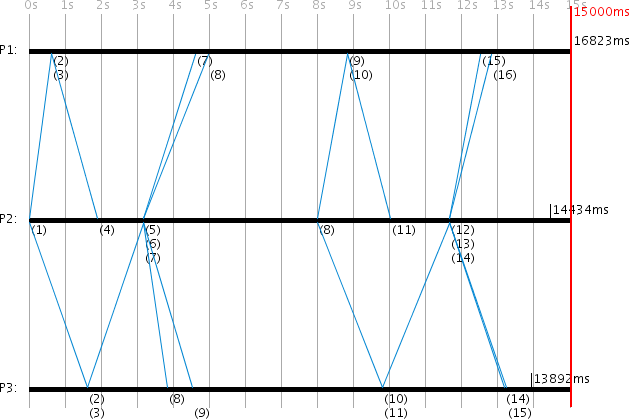
\includegraphics[width=10cm]{images/ss-protokoll-berkeley-lamport}}
	\caption{Lamportzeitstempel}
	\label{fig:Lamportzeit}
\end{figure}

Die Vektor- und Lamportzeitstempel lassen sich sehr gut am bereits behandelten Beispiel zum Berkeley-Protokoll demonstrieren. Nach Aktivierung der Lamportzeit-Checkbox erscheinen bei jedem Ereignis die zum jeweiligen Prozess geh\"{o}rigen Lamportzeitstempel (Abbildung \ref{fig:Lamportzeit}). Jeder Prozess besitzt einen eigenen Lamportzeitstempel, der bei jedem Versenden oder Erhalten einer Nachricht inkrementiert wird. Jeder Nachricht wird die aktuelle Lamportzeit $t_l(i)$ des sendenden Prozesses $i$ beigef\"{u}gt. Wenn ein anderer Prozess $j$ diese Nachricht erh\"{a}lt, so wird sein aktueller Lamportzeitstempel $t_l(j)$ wie folgt neu berechnet:

\begin{equation*}
	t_l(j) := 1 + max(t_l(j), t_l(i))
\end{equation*}

Es wird also stets die gr\"{o}ssere Lamportzeit vom Sende- und Empfangsprozess verwendet und anschlie�end um 1 inkrementiert. Nach Ablauf der Berkeley-Simulation hat P1 (16), P2 (14) und P3 (15) als Lamportzeitstempel. 

\begin{figure}[htbp]
	\centering
	\fbox{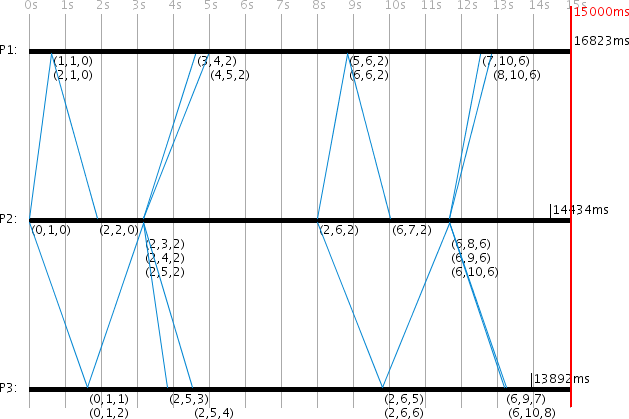
\includegraphics[width=10cm]{images/ss-protokoll-berkeley-vektor}}
	\caption{Vektorzeitstempel}
	\label{fig:Vektorzeit}
\end{figure}

Bei den Vektor-Zeitstempeln sieht es hier jedoch anders aus. Mit aktivierter Vektorzeit-Checkbox werden, wie auf Abbildung \ref{fig:Vektorzeit},  alle Vektor-Zeitstempel angezeigt.

